\documentclass{article}

% E&D Track, double-blind (default for the track)
\usepackage[eandd]{neurips_2026}

\usepackage[utf8]{inputenc}
\usepackage[T1]{fontenc}
\usepackage{hyperref}
\usepackage{url}
\usepackage{booktabs}
\usepackage{amsfonts}
\usepackage{amsmath}
\usepackage{amssymb}
\usepackage{nicefrac}
\usepackage{microtype}
\usepackage{xcolor}
\usepackage{graphicx}

\DeclareMathOperator*{\argmax}{arg\,max}

\newcommand{\dataset}{\textsc{CTSpinoPelvic1K}}
\newcommand{\TS}{TotalSegmentator}
\newcommand{\SOTA}{TotalSegmentator}
\newcommand{\sota}{TS}
\newcommand{\VERIDAH}{VERIDAH}
\newcommand{\VerSe}{VerSe}

\title{Not All Spines Are Created Equal: How TotalSegmentator\\
Fails on Lumbosacral Transitional Vertebrae}

\author{%
  Anonymous Author(s) \\
  Anonymous Affiliation \\
  \texttt{anonymous@institution.edu}
}

\begin{document}

\maketitle

% ============================================================================
\begin{abstract}
Wrong-level spine surgery remains a persistent
never-event, with the Lumbosacral Transitional Vertebra
(LSTV, 5--35\% prevalence) as its largest anatomic
driver. We audit \TS{}---the most widely deployed CT
segmentation system and default back-end of
3D~Slicer---and show that on lumbarization cases its
output is anatomically indistinguishable from a
wrong-level surgical plan: lacking an L6 class, it
shifts lumbar labels caudally by one level, with
junction-DSC dropping 29 points on Any-LSTV. No
existing CT benchmark surfaces this---not \TS{}'s own
evaluation, not \citet{Li2025LumbarMechanism} (the
per-class DSC frontier on the matched COLONOG split),
and not \VERIDAH{} (vertebra-\emph{labeling} SOTA on a
private CT cohort, operating on pre-localized crops
with no pelvis). We
contribute: (i)~an LSTV-stratified evaluation protocol
(per-class DSC, junction-DSC over a 40\,mm L5/S1
window, per-class voxel confusion at the junction)
translating the level-shift mechanism into quantifiable
wrong-level surgical risk;
(ii)~\dataset{}---1{,}153 CT volumes across 802
patients with unified spinopelvic masks, 33
LSTV-positive cases across a 6-way phenotype taxonomy,
and radiologist Castellvi typing (I--IV) on
all 33; (iii)~the first publicly-released
merge-based LSTV-handling dual-spinopelvic CT segmenter,
exceeding \TS{} on sacrum (\TS{}=0.817 zero-shot) and
uniquely delivering both spine and pelvis in a single
forward pass with released weights; (iv)~an empirical
isolation showing
\VERIDAH{}'s training-side L5/L6 merge eliminates the
collision driving \TS{}'s level shift but exposes a
residual L4/last\_lumbar collision on count-style
sacralization, motivating \VERIDAH{}'s sequence
predictor as the necessary disambiguation component.
\dataset{}, the protocol, and 5-fold checkpoints are
released publicly.
\end{abstract}

% ============================================================================
\section{Introduction}
\label{sec:intro}

Wrong-level spine surgery is a persistent never-event in
operative spine
care~\citep{Konin2010LumbosacralRelevance}. Despite
intraoperative imaging and surgical-pause checklists, the
most common cause---failure to correctly count vertebral
levels in the presence of an LSTV---continues to account for
the majority of reported wrong-level lumbar
incidents~\citep{Carrino2011EffectImaging}. The mechanism is
well documented: a surgeon counts lumbar bodies upward from
the sacrum, finds five (because lumbarization presents a
sixth lumbar body that has not been recognized), and labels
the bottom body as L5 when it is anatomically L6. Surgery
proceeds one level caudal to the intended target.

Modern radiology workflows increasingly route automated
segmentation as an upstream substrate for clinical
decision-making. The most widely deployed CT segmentation
system in this role is
\TS{}~\citep{Wasserthal2023TotalSegmentator:Images}: an
nnU-Net trained on 1{,}204 routine CTs to delineate 104
anatomic structures, the default segmentation back-end of
3D~Slicer, with thousands of clinical and research
installations. The original paper reports an aggregate
test-set Dice of 0.943 across all 104 classes and
qualitatively documents two spine failure modes
affecting neighboring-vertebrae label confusion (1\%
of cases) and neighboring-rib confusion (12\%). \TS{} is neither the
only public CT spine segmenter nor the per-class DSC
frontier on the matched CTSpine1K~+~CTPelvic1K (COLONOG)
split (\S\ref{sec:related}); it is, however, the model
surgeons and downstream tools consume. This paper
concerns one anatomic class on which \TS{} does not
perform at its headline level, and the consequences
when it does not.

\paragraph{The clinical claim.}
On lumbarized spines, \SOTA{} produces an output pattern
that is, when consumed by surgical planning pipelines or by
surgeons confirming operative levels, \emph{indistinguishable
from a wrong-level surgical plan}. Its label vocabulary
contains L1--L5 but no L6 class. On a lumbarized spine (six
lumbar bodies plus sacrum), the model distributes its five
lumbar labels across the six bodies by shifting caudally by
one anatomic level: the body that is anatomically L6
receives the L5 label, the body that is anatomically L5
receives the L4 label, and so on. A surgeon targeting the
disc between predicted-L4 and predicted-L5 lands on the
anatomical L5--L6 disc, one level caudal to the intended
L4--L5 target. \SOTA{} reproduces the canonical
LSTV-induced miscount automatically and silently.

\paragraph{The architectural alternative: \VERIDAH{}.}
Recent work~\citep{Moller2026VERIDAH:Sequences} addresses
transitional vertebra labeling via a two-stage
architecture: a 3D DenseNet169 classifier on per-vertebra
crops (four heads: label, region, transition, visibility),
followed by a constrained sequence predictor that imposes
anatomical-count constraints (4--6 lumbar bodies; the
predicted sequence may end in two consecutive L5 labels,
the second interpreted as L6). The classifier is trained
with L5/L6 (and T12/T13) labels merged for class-imbalance
reasons; disambiguation is deferred to the sequence
predictor. The architectural commitment is empirically
validated (97.22\% CT subject-level agreement) but has
never been tested against direct semantic segmentation,
and it is unknown whether a sufficiently expressive
voxel-wise network trained at full resolution with the
same merge requires the sequence predictor at all. We
supply the missing test.

\paragraph{The evaluation gap.}
Neither \SOTA{}, \VerSe{}~\citep{Sekuboyina2021VerSe:Images},
CTSpine1K~\citep{Deng2021CTSpine1K:Tomography}, nor
CTPelvic1K~\citep{Liu2021DeepModels} report LSTV-stratified
performance. Earlier CT labelers explicitly excluded the
failure mode~\citep{Sekuboyina2020LabelingAnatomy}.
\VERIDAH{} reports anomaly performance on a private cohort
without isolating semantic-segmentation contribution. The
result is a measurement vacuum: a production model emits a
confident, locally well-formed, caudally-shifted prediction
on a 5--35\%-prevalence congenital variant with no error
signal at evaluation time.

\paragraph{Closing the gap requires hardware.}
Fitting both lumbar spine and pelvis at
$0.75{\times}0.75{\times}0.80$\,mm spacing and
$256{\times}320{\times}320$ patch consumes ${\sim}100$\,GB
GPU memory under \texttt{nnUNetResEncUNetPlans\_100G},
available on H200 (140\,GB HBM3e) but not on the
L40S/A100/H100 GPUs that bracket \SOTA{}'s training
configuration. Neither \VERIDAH{} nor SPINEPS train at this
combined spinopelvic resolution.

\paragraph{Contributions.}
\begin{enumerate}
\item[(i)] \textbf{Wrong-level surgical risk in \sota{},
  quantified.} An LSTV-stratified evaluation protocol
  (per-class DSC, junction-DSC over a 40\,mm L5/S1
  window, per-class voxel confusion at the junction)
  measures \sota{}'s systematic one-level caudal shift
  on lumbarization (L4=0.388, L5=0.291; 95\%+ of GT-L6
  voxels labeled L5 on representative cases,
  \S\ref{sec:case_study}) and structural absence of L6
  prediction across all evaluation cases---translating
  the level-shift mechanism into quantifiable
  wrong-level surgical risk.
\item[(ii)] \textbf{\dataset{}: a stratified spinopelvic
  benchmark.} 1{,}153 abdominal CT records across 802
  patients, unified spinopelvic masks, 33 LSTV-positive
  patients across a 6-way subtype taxonomy
  (lumb $n=14$; sacr\_count $n=9$; full sacralization
  $n=6$; semi-sacralization $n=2$; ambiguous $n=2$), and a
  registration-free fusion pipeline that resolves a
  previously undocumented Y-axis coordinate-convention
  mismatch between CTSpine1K and CTPelvic1K. Both source
  datasets share the COLONOG cohort that underlies
  \VerSe{} and CTSpine1K, but neither encodes pelvic
  context with LSTV stratification. Radiologist
  Castellvi typing (I--IV) on all 33 LSTV cases is
  released as an additional annotation layer.
\item[(iii)] \textbf{First publicly-released merge-based
  LSTV-handling dual-spinopelvic CT segmenter.} A 5-fold CV nnU-Net
  3d\_fullres baseline on H200 hardware adopting
  \VERIDAH{}'s training-side merge
  (last\_lumbar = L5+L6) at the voxel level, with
  pelvic-class supervision in a single forward pass.
  We exceed \sota{} on sacrum and uniquely deliver both
  spine and pelvis with released weights
  (Table~\ref{tab:comparison}); \S\ref{sec:related}
  details the reproducibility tiers separating
  openly-released from paper-only baselines.
\item[(iv)] \textbf{Empirical isolation: merge alone is
  insufficient.} The merge eliminates the L5/L6
  collision driving \sota{}'s level shift but exposes a
  residual L4/last\_lumbar collision on count-style
  sacralization. This residual collision empirically
  isolates the component of \VERIDAH{}'s success
  attributable to its sequence predictor---a direction
  \VERIDAH{}'s authors could not ablate.
\end{enumerate}

% ============================================================================
\section{Related Work}
\label{sec:related}

\paragraph{Wrong-level spine surgery and LSTV.}
\citep{Konin2010LumbosacralRelevance,Carrino2011EffectImaging,Sekharappa2014LumbosacralSignificance}
document LSTV-induced miscounting (5--35\% prevalence) without
addressing automated segmentation as a miscount-propagation
pathway. \citet{Kwak2025AutomatedModel} detect LSTV on plain
radiographs (binary; different modality).

\paragraph{Transitional anatomy as one shift.}
The anatomical literature treats the thoracolumbar and
lumbosacral variants as two ends of one homeotic shift of
the column: a rib-less T12, a lumbar rib, a lumbarized S1
and a sacralized L5 are the same displacement read at
different
junctions~\citep{DuPlessis2018Homeotic,Poolman2023TransitionalVertebrae},
and twelfth-rib morphology co-varies with lumbosacral
status on CT~\citep{Nagata2025RibLSTV}. Stump ribs have
been detected automatically at
scale~\citep{Moller2025StumpRib}, but no public
segmentation benchmark labels both junctions on the same
spines, which is what a shift needs to be tested against.

\paragraph{Production CT spine and pelvic segmentation.}
\TS{}~\citep{Wasserthal2023TotalSegmentator:Images}, an nnU-Net
trained on 1{,}204 CTs and the default 3D~Slicer back-end,
has no L6 class and no LSTV stratification; we audit it as
the production system downstream pipelines actually consume,
not as a per-class DSC frontier.
\citet{Li2025LumbarMechanism} hold the published per-class
DSC frontier on a COLONOG split (731 scans; 440/146/145)
but release neither weights nor code (paper-only) and do
not stratify by LSTV. \citet{Liu2025AutomaticDataset}
release FracSegNet (PENGWIN+CTPelvic1K), a pelvic-only
cascaded 3D nnU-Net providing sacrum and L/R hipbone; their
qualitative note of sacralization degradation (their
\S4.3) corroborates the LSTV gap our benchmark surfaces.
Table~\ref{tab:comparison} compares all baselines.

\paragraph{Vertebra-labeling SOTA: \VERIDAH{}.}
\citet{Moller2026VERIDAH:Sequences} address transitional-vertebra
\emph{labeling} (distinct from segmentation): a four-head
3D DenseNet169 classifier on per-vertebra crops plus a
constrained sequence predictor enforcing 4--6 lumbar bodies
(allowing terminal double-L5 to encode L6). On a private
CT cohort of 1{,}536 volumes \VERIDAH{} reports 99.18\%
subject-level perfect labeling versus prior CT
SOTA~\citep{Meng2023VertebraeCycle} 77.81\%. Three
properties matter for us: \VERIDAH{} (i) requires upstream
centroids (\VerSe{}-derived models or
SPINEPS~\citep{Moller2024SPINEPSautomaticSegmentation},
itself MRI-only); (ii) excludes pelvis; (iii) validates on
a private CT cohort. Their ablation (Table~5) shows the
sequence predictor adds substantial value, but the
comparison against direct semantic segmentation on a
public LSTV-stratified split is missing---the gap our
\dataset{}-trained baseline (\S\ref{sec:baseline}) fills.

\paragraph{Benchmarks and evaluation rigor.}
\VerSe{}~\citep{Sekuboyina2021VerSe:Images} (460 CT volumes)
is the only public CT benchmark whose label vocabulary
includes L6 (label~25) but it is unstratified by LSTV and
lacks pelvic GT; earlier CT labelers explicitly excluded
the failure mode~\citep{Sekuboyina2020LabelingAnatomy}.
Stratified safety-critical
reporting~\citep{Maier-Hein2024MetricsValidation}
motivates~\S\ref{sec:protocol}.

% ============================================================================
\section{Failure-Mode Analysis: \sota{} on LSTV}
\label{sec:audit}

We evaluate \SOTA{} v2 (\texttt{total} task) zero-shot at
full resolution on the full \dataset{} matched cohort.
\SOTA{} was not trained on any \dataset{} case, so every
case is valid; this provides 1{,}152 of \dataset{}'s
1{,}153 records (one record dropped due to \sota{}
inference failure) aggregated to 801 patients via
patient-level merging, including 33 LSTV-positive
patients. Full-resolution mode isolates the failure as a
property of label vocabulary and training distribution
rather than inference resolution.

Table~\ref{tab:sota_stratified} reports performance by
phenotype. On normal anatomy ($n=768$) \SOTA{} performs at
its published level. On Any-LSTV ($n=33$) every metric
drops; lumbarization collapses caudally
(L1=0.878\,$\to$\,L4=0.388\,$\to$\,L5=0.291) with
junction-DSC at 0.357. Count-style sacralization ($n=9$)
collapses uniformly across all lumbar classes (L1=0.265
down to L5=0.000). \textsc{L6} predictions are
structurally zero across all 1{,}152 cases.

\begin{table}[t]
\caption{\dataset{} v10 composition. Counts are from the
released volumes and manifest; LSTV grades in
Table~\ref{tab:castellvi_dist}.}
\label{tab:scan_stats}
\centering
\small
\begin{tabular}{lc}
\toprule
\bfseries Property & \bfseries Value \\
\midrule
Records (one per patient)                         & 802 \\
\quad prone / supine                              & 377 / 425 \\
Label identifiers (contiguous, bone and hardware) & 68 \\
\quad vertebrae C1--L6 (\VerSe{} ids 1--25), sacrum, T13, S1 & 28 \\
\quad hips, femora                                & 4 \\
\quad ribs, thirteen per side                     & 26 \\
\quad lumbar ribs (left, right)                   & 2 \\
\quad hardware subtypes                           & 7 \\
Records with an L6                                & 18 \\
Records with a lumbar rib                         & 16 \\
Records with a stump twelfth rib (ratio $<0.33$)  & 98 \\
Four-lumbar records (fused segment carried as S1) & 9 \\
Instrumented records (hardware labelled)          & 11 \\
Castellvi-graded records (two-reader consensus)   & 33 \\
Ribs evaluable / residual offsets                 & 5{,}749 / 2 \\
\bottomrule
\end{tabular}
\end{table}

\begin{table}[t]
\caption{\sota{} zero-shot stratified by LSTV phenotype on
\dataset{}, full-resolution mode. Junction DSC over a
40\,mm L5/S1 axial window. \textsc{L6} count: cases with
any L6 voxel emitted (structurally zero by label
vocabulary). $\dagger$: junction analysis not computed for
separate-mode records.}
\label{tab:sota_stratified}
\centering
\small
\resizebox{\linewidth}{!}{%
\begin{tabular}{lrcccccccr}
\toprule
\bfseries Subgroup & \bfseries $n$ &
\bfseries L1 & \bfseries L2 & \bfseries L3 & \bfseries L4 & \bfseries L5 &
\bfseries Sac & \bfseries Hips &
\bfseries Jxn DSC \\
\midrule
All cases                              & 801 & 0.911 & 0.906 & 0.913 & 0.914 & 0.913 & 0.817 & 0.929 & 0.818 \\
Normal                                 & 768 & 0.921 & 0.918 & 0.929 & 0.936 & 0.938 & 0.817 & 0.929 & 0.824 \\
\midrule
Any LSTV                               & 33  & 0.681 & 0.615 & 0.523 & 0.367 & 0.314 & 0.822 & 0.929 & 0.534 \\
\quad Lumbarization                    & 14  & 0.878 & 0.853 & 0.690 & 0.388 & 0.291 & 0.833 & 0.928 & \textbf{0.357} \\
\quad Sacralization (count-style)      &  9  & 0.265 & 0.100 & 0.055 & 0.001 & 0.000 & 0.814 & 0.926 & 0.697 \\
\quad Semi-sacralization               &  2  & 0.951 & 0.951 & 0.951 & 0.955 & 0.956 & 0.824 & 0.937 & $\dagger$ \\
\quad Sacralization (full)             &  6  & 0.718 & 0.676 & 0.673 & 0.724 & 0.793 & 0.826 & 0.932 & 0.636 \\
\quad Ambiguous                        &  2  & 0.952 & 0.951 & 0.882 & 0.678 & 0.374 & 0.771 & 0.932 & $\dagger$ \\
\midrule
\textsc{L6 emit}                       &     &       &       &       &       &       &       &       & 0 / 1152 \\
\bottomrule
\end{tabular}%
}
\end{table}

\paragraph{The level-shift mechanism.}
The asymmetry between lumbarization (severe, caudally
progressive) and count-style sacralization (uniform
collapse) follows from a single fact: \SOTA{}'s output head
has no L6 class. For 6-vertebra anatomies the model
compresses 6 anatomic units into 5 labels by shifting label
assignment caudally; the most rostral body remains L1
(escape into thoracic vertebrae), but every successive body
is misaligned, with the final body labeled L5 when it is
anatomically L6. For 4-vertebra anatomies the model emits
standard L1--L5, overshooting the GT lumbar count and
producing a $+1$-level offset uniformly. The level-shift
mechanism is the segmentation analog of the surgical
miscount~\citep{Konin2010LumbosacralRelevance}.

% ============================================================================
\section{Case Study: Wrong-Level Surgical Risk in \sota{}
Output}
\label{sec:case_study}

Aggregate metrics establish the population pattern; the
case study below establishes the mechanism at the level a
surgeon would consume the output. Token~215 is a
lumbarization case (six anatomical lumbar bodies, separate
spine and pelvic GT records merged at patient level).
\sota{}'s output head emits only L1--L5, so on a 6-vertebra
anatomy the bottom-most body (anatomical L6) cannot receive
its correct label. Table~\ref{tab:case215} reports
per-class DSC: L1 and L2 are well-placed
($0.954$, $0.927$), L3 is partially correct ($0.594$),
and \textbf{L4, L5, and L6 all collapse to dice~zero}---a
clean signature of the level-shift, with no GT-L4 voxel
correctly labeled, no GT-L5 voxel correctly labeled, and no
L6 voxel emitted at all. The pelvic classes (sacrum, hips)
remain at near-Normal accuracy, confirming that the failure
is local to the lumbosacral count and not a general
degradation of \sota{} on this patient.

\begin{table}[h]
\caption{Token~215 (lumbarization, 6 lumbar bodies):
per-class \sota{} zero-shot DSC. The L4--L5--L6 row is the
empirical signature of the level-shift failure---all three
collapse to dice zero because \sota{} compresses 6 anatomical
bodies into 5 labels. Pelvic classes are unaffected.
$\dagger$~\sota{}'s output head has no L6 label.}
\label{tab:case215}
\centering
\small
\begin{tabular}{lccccccccc}
\toprule
\bfseries Class & L1 & L2 & L3 & L4 & L5 & L6 & Sacrum & Hip$_L$ & Hip$_R$ \\
\midrule
\bfseries DSC & 0.954 & 0.927 & 0.594 & \textbf{0.000} & \textbf{0.000} & \textbf{0.000}$^{\dagger}$ & 0.817 & 0.922 & 0.926 \\
\bottomrule
\end{tabular}
\end{table}

\begin{figure}[h]
\centering
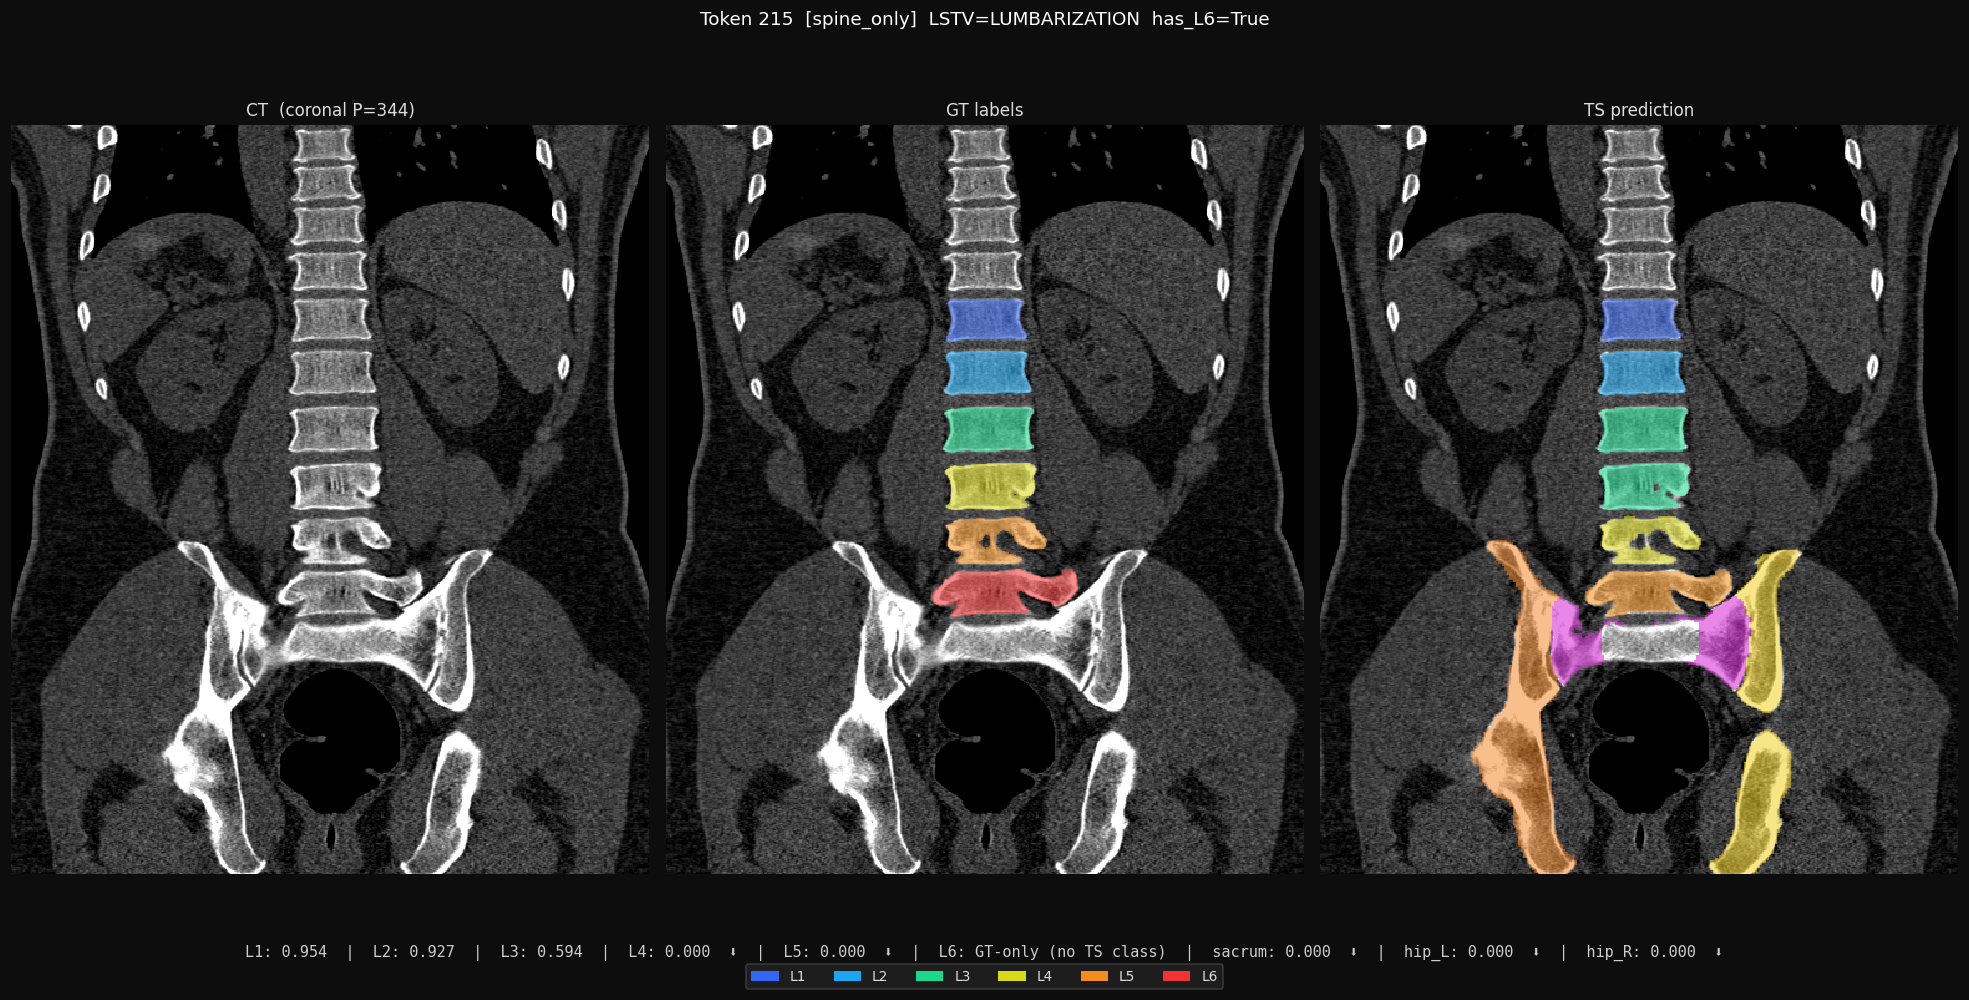
\includegraphics[width=\linewidth]{figs/lstv_lumbarization_215_spine_only.png}
\caption{Token~215, lumbarization case (6 anatomical lumbar
bodies). \sota{} predictions overlaid on CT. The model
compresses 6 bodies into 5 lumbar labels with a caudal
cascade: the predicted-L3 region absorbs both anatomical
L3 and L4 (yielding partial L3 dice 0.594, zero L4 dice);
predicted-L4 sits over anatomical~L5 (zero L5 dice);
predicted-L5 sits over anatomical~L6 (which has no label
in \sota{}'s output head; zero L6 dice). The output is
locally well-formed---five compact vertebral predictions
in approximately correct positions---but every label below
L2 is one anatomical level off, with the bottom body
unlabeled-as-L6 entirely. Quantified in
Table~\ref{tab:case215}.}
\label{fig:case215}
\end{figure}

\paragraph{Surgical translation.}
A surgeon planning an L4--L5 microdiscectomy and using the
segmentation to confirm operative level identifies the
disc between predicted-L4 (anatomical L5) and predicted-L5
(anatomical L6). The targeted disc is L5--L6, one level
caudal to the L4--L5 intent. The output is locally
well-formed: five compact vertebral predictions in roughly
correct positions. The error is detectable only by
counting bodies (six lumbar, not five), which downstream
pipelines do not perform.

% ============================================================================
\section{\dataset{}: Construction and Composition}
\label{sec:dataset}

\dataset{} fuses CT scans from
COLONOG~\citep{Smith2015DataCOLONOGRAPHY} with annotations
from CTSpine1K~\citep{Deng2021CTSpine1K:Tomography}
(\VerSe{}-derived per-vertebra masks) and
CTPelvic1K~\citep{Liu2021DeepModels} (sacrum and bilateral
hips). The same COLONOG cohort underlies \VerSe{} and
CTSpine1K; \dataset{}'s contribution is the patient-level
fusion of CTSpine1K's vertebra masks with CTPelvic1K's
pelvic masks, on one series per patient, plus the anatomy
neither source labelled and the LSTV-stratification
overlay neither provides. The release described here is
v10 (September 2026): 802 records, one per patient, each
on the patient's bone-richest acquisition; the 351
patients whose spine and pelvis were annotated on two
different acquisitions are held out as a paired
prone/supine resource rather than merged
(Table~\ref{tab:scan_stats}).



\paragraph{What was added to the source annotations.}
Every record carries, beyond the CTSpine1K vertebrae and
the CTPelvic1K sacrum and hips: per-level ribs on each
side, a thirteenth-rib class per side so a rib borne by a
T13 is not forced to be a twelfth, left and right lumbar
ribs as their own classes so a rib borne by a lumbar body
is not forced to be a twelfth either, both femora, a first
sacral segment carved from the sacrum as the caudal anchor,
and surgical hardware as its own class family (generic,
cage, screw--rod, plate, arthroplasty, iliosacral screw,
osteosynthesis). Lumbar levels are anchored on the lowest
rib-bearing vertebra and on S1 rather than on a count, so
a sixth lumbar body, a thirteenth thoracic body, a stump
rib and a lumbar rib are recorded as what they are. The
ribs began as model output (TotalSegmentator numbering
completed by the M\"oller rib network) and were then
reviewed by thirteen trained student annotators under a
triaged protocol; the thoracic column added the same way.
The release passes three validation layers: per-record
geometric invariants (802 of 802), rib--vertebra incidence
across 5{,}749 evaluable ribs (2 residual offsets,
0.035\%), and agreement of derived spinopelvic measures
with published reference values. The full build chain,
from the public sources through every non-regenerable
intermediate (source placements, the model-output base the
students corrected, the review ledgers, the hand
corrections, the radiologist hardware reads) to the
released volumes, is archived separately
(Zenodo 10.5281/zenodo.22647933) with a check that the
final scripted hops regenerate the release voxel for voxel.

\paragraph{Patient-anchored fusion and coordinate
correction.} Patient identity is resolved via canonical UID
matching (825/825 patients). Each mask is assigned to its
source CT acquisition by intra-patient bone-HU
maximization,
$s^*(m) = \argmax_{s \in \mathcal{S}_p}
|\{v \in \mathcal{L}(m, s) : I_s(v) > 200\,\text{HU}\}|/|\mathcal{L}(m, s)|$,
a metadata-free oracle since \texttt{SeriesDescription}
fields are unreliable in TCIA releases (99.6\% spine,
100\% pelvic placement). CTSpine1K and CTPelvic1K were
converted from DICOM with different \texttt{dcm2niix}
invocations, producing a systematic Y-axis sign reflection
in NIfTI affines; we detect via affine-derived center sign
and reverse along axis~1 with affine update. The
released volumes keep the \VerSe{}-native vertebral
identifiers (L6\,=\,25, so an L6 here is interoperable with
\VerSe{} and CTSpine1K) in a contiguous 68-identifier
scheme; the merged last\_lumbar scheme of
\S\ref{sec:baseline} and the one-shot scheme of
\S\ref{sec:oneshot} are training-time remaps of that
release, produced by one converter, never edits to it.

\paragraph{Six-way LSTV taxonomy with dual-origin
labels.} We retain both LSTV label sources separately and
partition into six subtypes by combining filename-qualifier
evidence (CTPelvic1K morphological criterion) with
vertebral-counting evidence (CTSpine1K
\VerSe{}-label-presence heuristic):
\textbf{normal}, \textbf{lumb} (6 vertebrae labeled or
\VerSe{} label 25 present), \textbf{sacr\_count} (4
vertebrae labeled with sacralization flag),
\textbf{semisacralization}, \textbf{sacralization}
(both via filename qualifier), and \textbf{ambiguous}
(cross-source disagreement). An earlier substring-match
parser bug collapsed semisacralization into full
sacralization---merging two anatomically distinct
phenotypes whose failure modes diverge sharply (full
sacralization preserves the lumbar count and produces
near-normal per-class DSC, whereas semisacralization
introduces a partial transition that confuses the L5/S1
boundary). Any benchmark reporting an aggregate
sacralization DSC under this collapse averages over
two qualitatively different model behaviors; we identify
and fix this. Without the corrected 6-way taxonomy, the
qualitatively different failure patterns across LSTV
variants (\S\ref{sec:audit}) are invisible.

\paragraph{Partial-annotation training protocol.}
\label{sec:partial}
Training only on fused records discards 70\% of the data.
We use nnU-Net v2's
\texttt{ignore\_label}~\citep{Isensee2024Nnu-netSegmentation}
to train on all 1{,}153: voxels in unsupervised regions are
written as label~9, contributing zero to Dice and
cross-entropy. Spine classes (1--5) receive supervision
from 784 records; pelvic classes (6--8) from 714. This is a
$3.36\times$ effective expansion. Per-record subtype
refinement gates training-time tags on supervised anatomy.

\paragraph{Castellvi annotation layer.}
\label{sec:castellvi}
The 6-way taxonomy captures the \emph{count} dimension of
LSTV. The Castellvi
classification~\citep{Castellvi1984LumbosacralDefects}
captures the orthogonal \emph{morphological} axis:
Type~I (dysplastic transverse process), II
(pseudoarticulation), III (bony fusion), or IV (mixed
II/III), each \texttt{a}~(unilateral) or
\texttt{b}~(bilateral). It is the surgeon's
pre-operative wrong-level-risk indicator, and what a CT
segmenter would need to predict to flag LSTV for review
rather than silently emit a caudally-shifted label.
Two resident radiologists jointly annotated all 33 LSTV
cases by consensus (no independent inter-rater scoring),
extending the schema---originally
sacralization-specific---to score the bony junction
uniformly across variants, with per-side
\texttt{a}/\texttt{b} laterality.

\begin{table}[h]
\caption{Castellvi distribution across all 33 LSTV cases
of \dataset{}, cross-tabulated by 6-way count taxonomy.}
\label{tab:castellvi_dist}
\centering
\small
\setlength{\tabcolsep}{4pt}
\begin{tabular}{lrrrrrrrr}
\toprule
\bfseries Subtype & \bfseries Ia & \bfseries Ib & \bfseries IIa & \bfseries IIb & \bfseries IIIa & \bfseries IIIb & \bfseries IV & \bfseries Total \\
\midrule
Lumbarization                  & 0 & 1 & 1 & 3 & 1 & 7 & 1 & 14 \\
Sacralization (count-style)    & 0 & 0 & 0 & 0 & 0 & 9 & 0 & 9 \\
Sacralization (full)           & 0 & 0 & 0 & 0 & 1 & 3 & 2 & 6 \\
Semi-sacralization             & 0 & 0 & 1 & 0 & 1 & 0 & 0 & 2 \\
Ambiguous                      & 0 & 0 & 0 & 1 & 0 & 0 & 1 & 2 \\
\midrule
Total                          & 0 & 1 & 2 & 4 & 3 & 19 & 4 & 33 \\
\bottomrule
\end{tabular}
\end{table}

\paragraph{Morphology-stratified failure interpretation.}
The cross-tabulation (Table~\ref{tab:castellvi_dist})
surfaces two findings with direct bearing on model
behavior. (1)~\textbf{All 9 count-style sacralization
cases are Castellvi~IIIb}---bilateral bony fusion---and
19/33 (58\%) of LSTV overall is IIIb. The residual
L4/last\_lumbar collision (\S\ref{sec:residual})
therefore occurs precisely when the discriminating cue
is locally observable: bony fusion of the bottom lumbar
to sacrum is visually distinct from a normal L5--S1
junction, yet the segmenter still emits last\_lumbar
for those voxels. Direct semantic segmentation has not
learned the Castellvi correlate of the count anomaly
even when it is morphologically present in the input.
That is the empirical case for the one-shot arm of
\S\ref{sec:oneshot}, which names the border bodies by
type from their own appearance and leaves the count to a
decoder, rather than for a global count constraint that
would inherit the same ambiguity. (2)~Only 1/33 cases is Type~I
(population prevalence
14--16\%~\citep{Sekharappa2014LumbosacralSignificance}),
reflecting source-dataset selection bias toward
morphologically conspicuous presentations. Reported
performance therefore characterizes the conspicuous
regime; the clinically subtler Type~I fraction is
uncharacterized in this benchmark.

% ============================================================================
\section{Evaluation Protocol}
\label{sec:protocol}

We define four metrics as the minimum required to attribute
LSTV failure modes to wrong-level surgical
risk~\citep{Maier-Hein2024MetricsValidation}: (1) per-class
DSC stratified by 6-way LSTV subgroup, exposing class-level
degradation; (2) junction-DSC over a 40\,mm L5/S1 axial
window, the clinical window for surgical planning;
(3) per-class voxel confusion at the L5/S1 junction, which
exposes structured failure modes (the level shift) that
DSC alone cannot characterize; and (4) for the merged-label
baseline, three focused per-epoch confusion blocks anchored
on the L4/last\_lumbar boundary that drives the residual
collision (\texttt{last\_lumbar\_GT\_on\_lumb},
\texttt{L4\_GT\_on\_sacr\_count},
\texttt{pred\_last\_lumbar\_on\_sacr\_count}) plus a
specificity number
(\texttt{last\_lumbar\_specificity\_on\_sacr\_count}).

\paragraph{The one-shot arm and the competitors are scored
in one space.} For the one-shot arm (\S\ref{sec:oneshot})
and for every public system we compare against, the unit
of evaluation is the same: the 22-class one-shot labels of
all 802 records, our own network on its validation fold,
each competitor on all 802 (none was trained on them).
Every competitor's native output is mapped into that space
by class name, ribs one to eleven pooled per side, its
sacrum and S1 classes unioned onto our whole sacrum, its
femora pooled, and anything above T10 sent to background,
where our labels are ignore in any case. Four numbers are
then read off with the same code for every system: per-class
Dice on typical and on transitional records separately;
the rib-free count and its exact-match rate by transitional
status; where the ground-truth twelfth-rib, thirteenth-rib
and lumbar-rib voxels went; and whether the rare classes
(L6, T13, the lumbar ribs) are emitted at all on the
records that carry them. Hard-label systems pass through the
sequence decoder as one-hot, so a system without an L6
class still has its \emph{count} scored fairly, since two
touching bodies with one name are split, while its
\emph{name} is scored as the miss it is. The systems:
TotalSegmentator v2 (\texttt{total} task, full resolution,
no region subset so that no second model crops the
input)~\citep{Wasserthal2023TotalSegmentator:Images};
SPINEPS-CT with the VERIDAH labeling head, the one
competitor that can name an L6 and a
T13~\citep{Moller2024SPINEPSautomaticSegmentation,Moller2026VERIDAH:Sequences},
with M\"oller's rib network and rib-assignment code beside
it~\citep{Moller2025StumpRib}; NV-Segment-CT, the released
VISTA3D lineage; and RibSeg~v2 for rib numbering.
\textbf{[PENDING: numbers; runs launched 8 September
2026.]}

% ============================================================================
\section{Spinopelvic Baseline}
\label{sec:baseline}

\paragraph{Architecture and training.}
nnU-Net v2~\citep{Isensee2020NnU-Net:Segmentation,Isensee2024Nnu-netSegmentation}
ResEnc-M planner, \texttt{3d\_fullres},
\texttt{nnUNetResEncUNetPlans\_100G} (100\,GB GPU budget).
Spacing $0.80{\times}0.75{\times}0.75$\,mm, patch
$\mathbf{256{\times}320{\times}320}$, batch~2; 7-stage
residual encoder
($n_\text{features}{=}[32,64,128,256,320,320,320]$,
$n_\text{blocks}{=}[1,3,4,6,6,6,6]$, $3^3$ kernels, $2^3$
strides, instance norm, deep supervision at 5 levels);
9-channel output (bg + 8 fg); ignore-label masked from
loss. Class-reweighted DC\_and\_CE loss
($\mathbf{w}{=}[0.5,1,1,1,1,\mathbf{1.5},\mathbf{2.0},1,1]$;
last\_lumbar boost targets the clinically-important
boundary, sacrum boost supports Castellvi precision); SGD
Nesterov 0.99, $\lambda{=}3{\times}10^{-5}$, PolyLR
$10^{-2}$, 500 epochs (250 train + 50 val iters); 5-fold
patient-stratified CV with 6-way LSTV stratification.

\paragraph{Two-tier LSTV emphasis.}
\textbf{Queue-level oversampling}: all five non-normal
subtypes duplicated to 25\% of per-fold training samples
(matching \VERIDAH{}'s 4$\times$ rate).
\textbf{Class-reweighted CE} (above). No per-patch
foreground biasing: under merged labels, biasing toward
an L6 class is ill-defined, and biasing the
L4/last\_lumbar boundary on sacr\_count would confound
the residual-collision measurement.

\paragraph{Hardware.}
H200 NVL (140\,GB HBM3e), 24 CPU workers, preunpacking
once per job to a 1.7\,TB local-NVMe cache (replacing NFS
reads that throttled at 21\,MB/s under 5-fold contention).
Per-epoch ${\approx}\,400$--$700$\,s; per-fold
${\approx}\,3$ days for 500 epochs. Reducing the GPU memory
budget forces either smaller patch (loses spinopelvic
context) or coarser spacing (loses Castellvi-defining
detail); 100\,GB is the smallest budget fitting both.

% ============================================================================
\section{One-Shot Level Identity and the Sequence Decoder}
\label{sec:oneshot}

The merged baseline of \S\ref{sec:baseline} closes the
level-shift gap by construction: it refuses to name L5
and L6 apart, so it can never shift them. That is the
right engineering answer for a segmenter that must not
mislead a surgeon, and the wrong instrument for the
scientific question the residual collision raises
(\S\ref{sec:residual}): whether a vertebra's identity is
\emph{locally} decidable at all. The one-shot arm asks the
network to name every level from its own appearance, with
no count anywhere in the target, and then adds the one
thing a semantic network cannot supply, the reasoning
about the sequence.

\paragraph{The premise, tested before a GPU was spent.}
If T12 and L1 were not different shapes, a local
classifier could only learn the annotators' convention.
On the released morphometrics, eleven shape features per
vertebra, each divided by the patient's own median across
levels so that size is removed and only shape remains,
separate thoracic from lumbar at AUC~0.998 and T12 from
L1 at AUC~0.990 (accuracy 97.3\% over 1{,}485 vertebrae,
plain logistic regression, cross-validated by patient).
Transverse-process span carries most of the weight;
costal facets and facet-joint orientation are not in the
feature set at all, and a network sees them directly.

\paragraph{Target.} The release is remapped to 43
foreground classes plus ignore (Dataset813): T10, T11,
T12 and T13 as distinct thoracic classes; L1--L6 as
distinct lumbar classes; the sacrum; every rib named per
side, one to thirteen, with the lumbar rib as its own
class per side; the hips; the femora; and one derived
class, the intervertebral space, computed at conversion
from the per-level source labels wherever two consecutive
bodies are both present. The lumbosacral disc is
deliberately not derived, since whether one exists is the
transitional finding. With the disc as a class, every
vertebra is its own connected component of the vertebra
classes, so an instance can carry one name only, by
construction of the decoding rather than by hope. The
twelfth rib and the lumbar rib are separate classes
because that pair \emph{is} the discrimination under
test, and L5 is kept apart from L6 because whether the
network can tell them apart is the question rather than
a nuisance. An earlier arm with ribs one to eleven pooled
(22 classes, Dataset810) was retired at epoch~35 once it
had shown L6 learned as its own class
(Fig.~\ref{fig:training}); the numbered-rib arm keeps
every property of it and adds the ribs.

\begin{figure}[t]
\centering
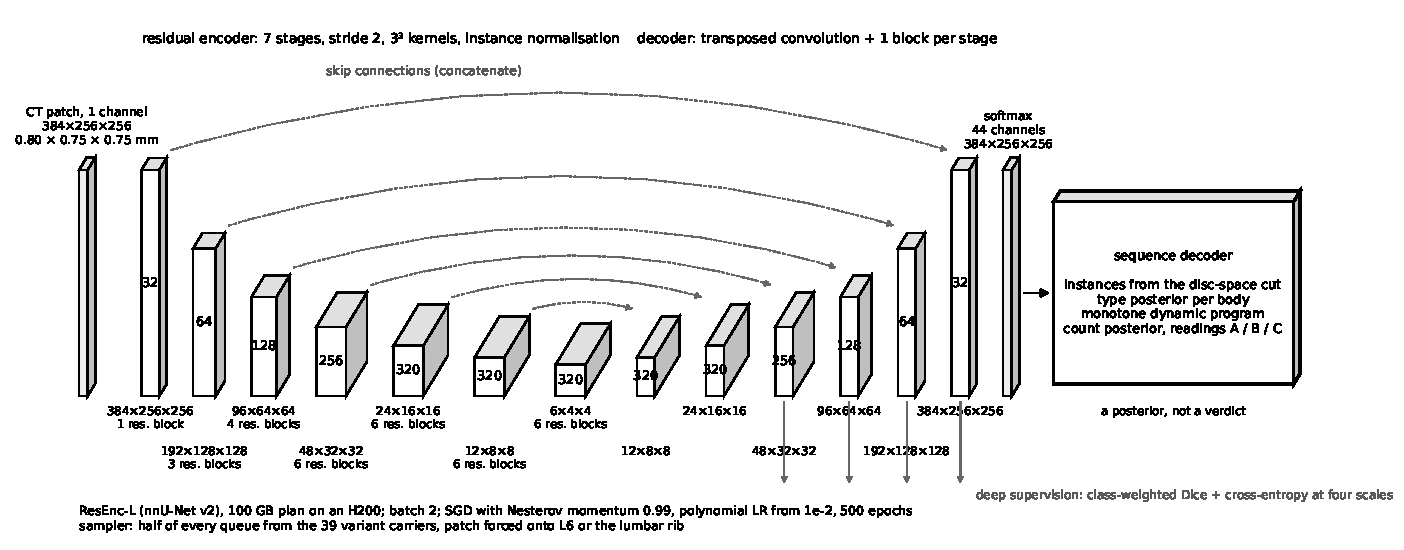
\includegraphics[width=\linewidth]{figs/fig_architecture.pdf}
\caption{The network. A seven-stage residual encoder
(channels 32 to 320, one to six residual blocks per
stage) and a mirrored decoder with skip connections and
deep supervision, a 44-way softmax, and the sequence
decoder that turns voxels into a count with a posterior.
Boxes are labelled with channels; spatial extents below.}
\label{fig:architecture}
\end{figure}

\paragraph{Sampler.} nnU-Net's foreground oversampling
picks a class inside an already-selected case, and case
selection is uniform, so a class present in 16 of 802
records is seen a fraction of a percent of the time and is
learned, correctly by its loss, as never to be predicted.
Two changes address that: records carrying any variant
(lumbosacral subtype, a lumbar rib, a T13) are drawn to
half of every training queue, and inside such a record
the patch is forced onto the rare class (the lumbar rib
where present, else L6) with probability 0.6. Class
weights in the cross-entropy term are 3.0 for L6 and the
lumbar ribs, 2.5 for T13 and the thirteenth ribs, 2.0 for
the twelfth ribs, 1.5 for T12, L5 and the sacrum, 1
elsewhere, 0.5 for background.

\paragraph{Architecture and training.} nnU-Net v2
ResEnc-L, \texttt{3d\_fullres}, 100\,GB memory target
(Fig.~\ref{fig:architecture}). The planner's patch,
$256{\times}320{\times}320$ voxels at
$0.80{\times}0.75{\times}0.75$\,mm, spans 20.5\,cm along
the column; counting needs T10 to the sacrum, about
30\,cm. The patch was therefore reshaped to
$384{\times}256{\times}256$, 30.7\,cm along the column and
19.3\,cm in-plane, at the same voxel budget (25.2 against
26.2 million) and the same batch of two on an H200. The
choice is measured, not argued
(Fig.~\ref{fig:patch-context}): over all 802 label volumes,
a window of the planner's shape centred on the column holds
5.1 whole vertebral levels, 3.6\% labelled voxels, and both
counting anchors, the sacrum and a rib-bearing body, in
30\% of scans; the column-shaped window holds 9.5 levels,
6.6\% labelled voxels, and both anchors in 98\%. Placed on
the lumbosacral junction, where the sampler puts the
rare-class patches, both shapes see the anchors (99\%) but
the column shape still holds nine whole levels to the
planner's five. The price is the iliac wing, which the
column shape clips; the hips are learned from the patches
the sampler places on them. A longer shape,
$448{\times}224{\times}224$, gains little more (9.6 levels)
and cuts the pelvis harder. All three, and a
$512{\times}192{\times}192$ extreme, train on one fold as
an ablation; the shape reported here is the one the
validation curves select \textbf{[PENDING]}.

\begin{figure}[t]
\centering
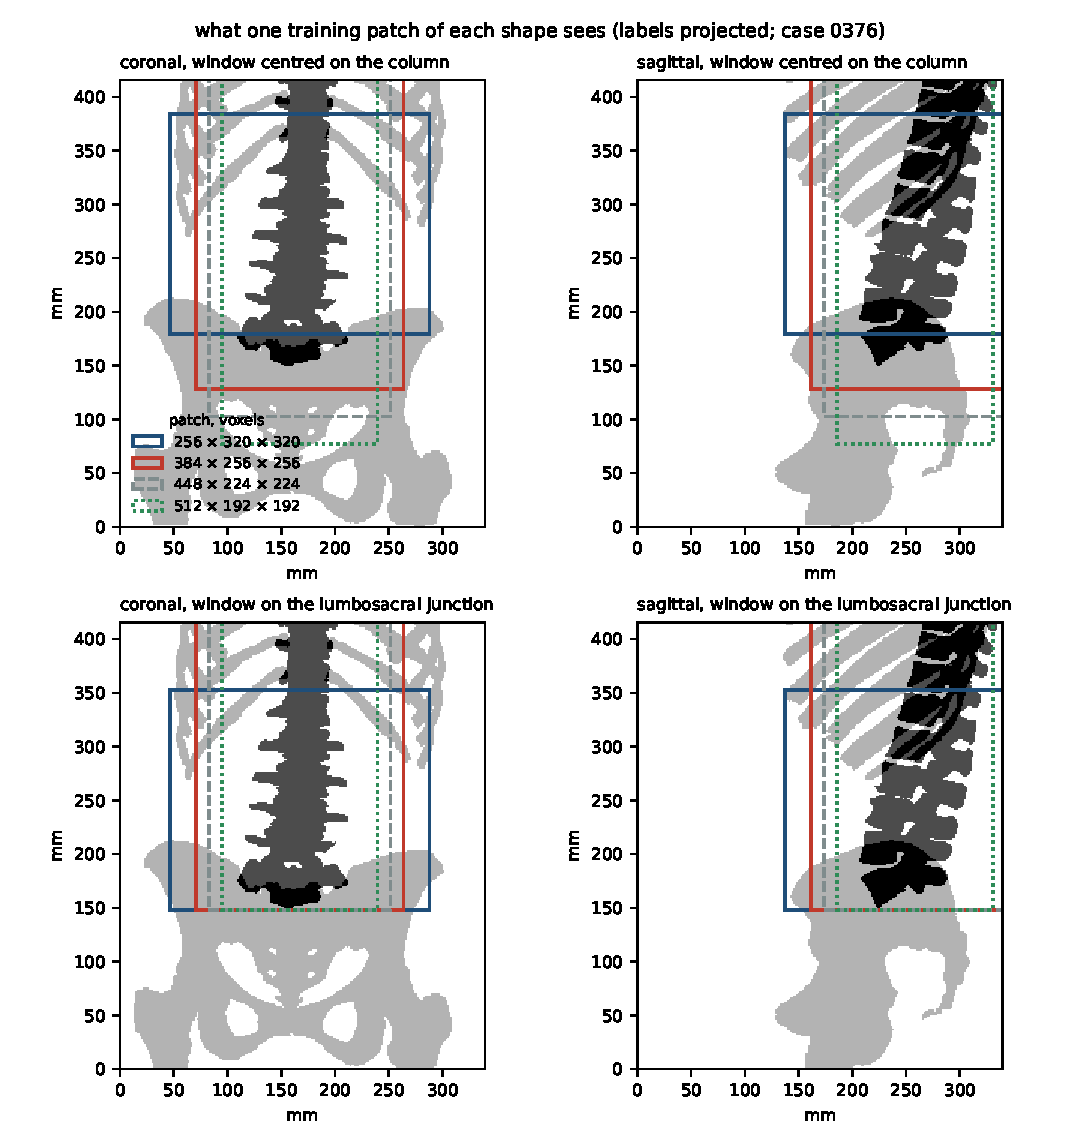
\includegraphics[width=0.9\linewidth]{figs/fig_patch_context_0376.pdf}
\caption{One training patch of each shape on a six-lumbar
spine, labels projected coronally and sagittally, centred
on the column (top) and on the lumbosacral junction
(bottom). The planner's square patch ends at the sacral
promontory; the column shapes reach from T10 through the
sacrum and clip the iliac wings.}
\label{fig:patch-context}
\end{figure} The same five patient-grouped LSTV-stratified folds
as the baseline, 500 epochs per fold, reading the
preprocessed volumes from the shared filesystem after a
single unpack. Validation predictions are written with
their softmax probabilities.

\paragraph{Decoder.} A semantic network can output
``T12, L1, T12, L2'' for four consecutive bodies. The
decoder adds only the anatomical constraint and nothing
learned. Vertebra instances are the connected components
of each name class, with same-name fragments within a body
height merged. For each instance the mean softmax over its
voxels is folded into three type probabilities, thoracic
(T10--T13), lumbar (L1--L6) and sacral, and a most likely
name; rib classes within 4\,mm are recorded. Ordering
instances from superior to inferior, the boundary $k$
between thoracic and lumbar is chosen to maximise the
summed log type probability, and the softmax of that
score over $k$ is a posterior over the rib-free count.
When the most likely count is six, the three readings of
\S\ref{sec:intro} are scored: B (a rib-less T12 counted
as lumbar) is the posterior mass on $k{+}1$; C (a
lumbarized S1) is the sacral share of the lowest
instance's type mass; A is the remainder; and the double
shift, both at once, is reported as their product rather
than excluded. On one-hot ground truth the decoder
reproduces the label's rib-free count on every record
tested, which establishes the instance handling and the
axis conventions before any network output exists.

\begin{figure}[t]
\centering
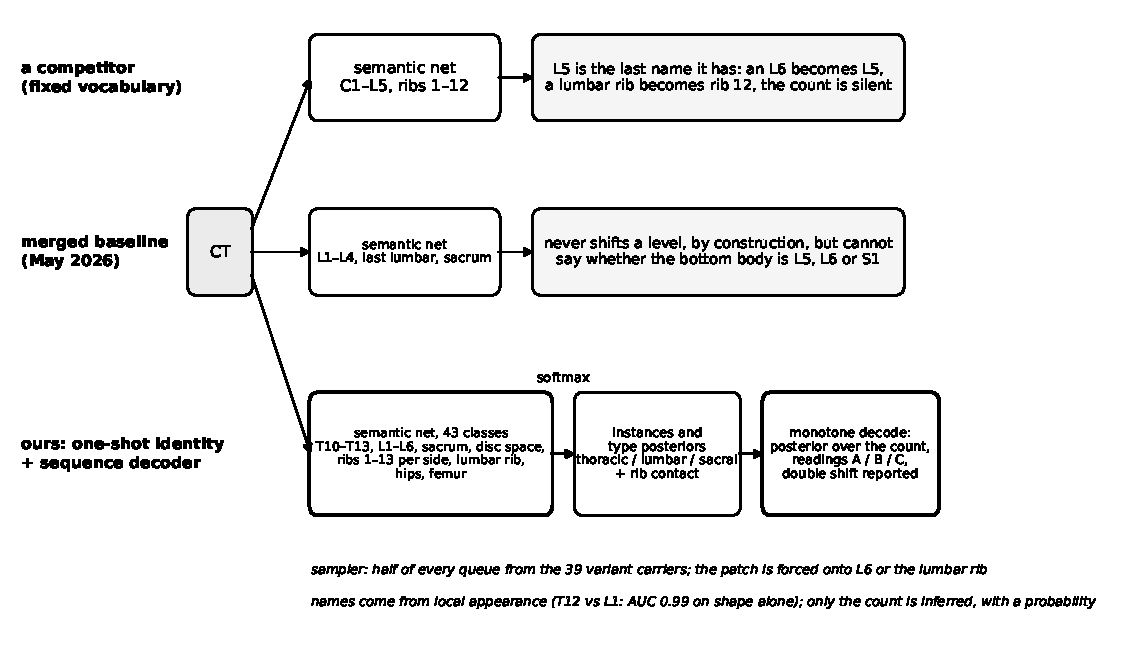
\includegraphics[width=\linewidth]{figs/fig_pipeline_oneshot.pdf}
\caption{Three ways to read a column. A fixed-vocabulary
competitor and our merged baseline each stop where their
names stop. The one-shot arm names every level from its
own appearance and hands the count to a decoder that
returns a posterior.}
\label{fig:pipeline-oneshot}
\end{figure}

\begin{table}[t]
\centering
\caption{What each system can say about a spine. Filled:
a class or output the released system produces. Open: in
the released labels; the arm that names every rib per
side (Dataset813) is queued behind the one-shot folds.}
\label{tab:capabilities}
\small
\begin{tabular}{lccccc}
\toprule
 & TotalSeg.~v2 & NV-Segment-CT & SPINEPS+VERIDAH & RibSeg~v2 & \textbf{ours} \\
\midrule
vertebrae T10--L5 by name & $\blacksquare$ & $\blacksquare$ & $\blacksquare$ &  & $\blacksquare$ \\
sacrum (and S1) & $\blacksquare$ & $\blacksquare$ & $\blacksquare$ &  & $\blacksquare$ \\
hips and femora & $\blacksquare$ & $\blacksquare$ &  &  & $\blacksquare$ \\
ribs, numbered per side & $\blacksquare$ & $\blacksquare$ &  & $\blacksquare$ & $\blacksquare$ \\
twelfth rib as its own class & $\blacksquare$ & $\blacksquare$ &  & $\blacksquare$ & $\blacksquare$ \\
a rib on L1 (lumbar rib) &  &  &  &  & $\blacksquare$ \\
a sixth lumbar body (L6) &  &  & $\blacksquare$ &  & $\blacksquare$ \\
a thirteenth thoracic body (T13) &  &  & $\blacksquare$ &  & $\blacksquare$ \\
voxel probabilities released &  &  &  &  & $\blacksquare$ \\
posterior over the rib-free count &  &  &  &  & $\blacksquare$ \\
readings A / B / C for six bodies &  &  &  &  & $\blacksquare$ \\
trained on labelled transitional anatomy &  &  & $\blacksquare$ &  & $\blacksquare$ \\
public CT test set with LSTV strata &  &  &  &  & $\blacksquare$ \\
\bottomrule
\end{tabular}

\end{table}

\begin{figure}[t]
\centering
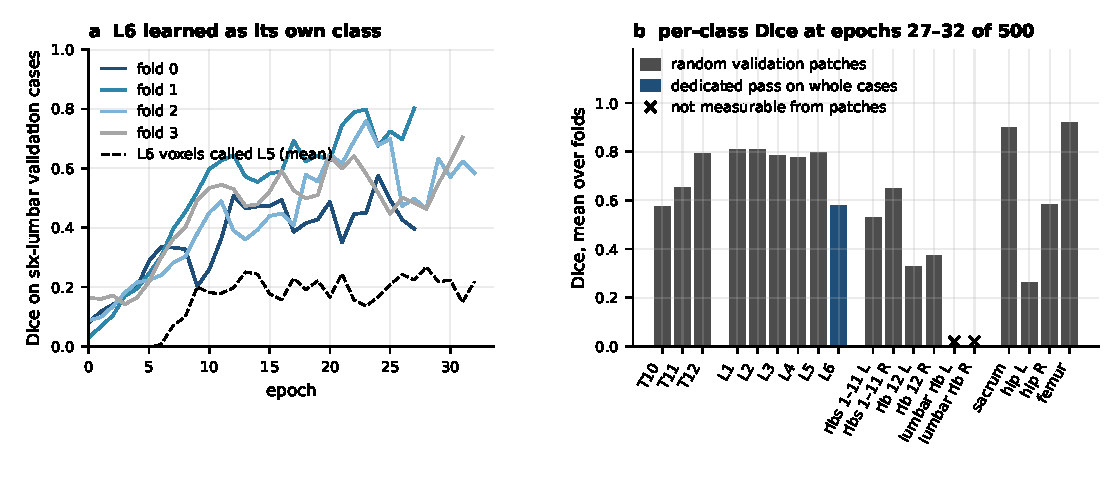
\includegraphics[width=\linewidth]{figs/fig_training.pdf}
\caption{Training-time evidence, four folds, first
thirty epochs of 500. (a)~L6 Dice on the six-lumbar
validation records from the dedicated pass, against the
fraction of L6 voxels called L5. (b)~Per-class Dice at
the latest epoch; the lumbar ribs are not measurable from
random validation patches.}
\label{fig:training}
\end{figure}

\paragraph{Every rib named.} The released labels number
thirteen ribs per side. The one-shot arm pools ribs one to
eleven to spend its capacity at the junction; a second
arm with the same sampler and every rib as its own class
(42 foreground classes, Dataset813) is queued so that no
public system numbers ribs where ours does not
(Table~\ref{tab:capabilities}). \textbf{[PENDING]}

\paragraph{What it cannot do.} The names L5 and L6 are
a count; the decoder does not pretend otherwise. What it
decides is the \emph{type} of each border body, and the
posterior it reports is the honest output on a study
that contains no C2.

% ============================================================================
\section{Results}
\label{sec:results}

\paragraph{Headline.}
The merged-label spinopelvic baseline closes the LSTV
junction-DSC gap on lumbarization: junction-DSC rises
from \sota{}\,=\,$0.357$ to ours\,=\,$\textbf{0.946} \pm
0.007$ (5-fold mean $\pm$ std; ensemble $0.950$), a
$\Delta{=}\,\textbf{+58.9} \pm 0.7$~points (5-fold;
ensemble $+59.3$~points). The model emits non-degenerate
last\_lumbar on all 3/3 held-out lumbarization test
cases with per-case last\_lumbar DSC of
$0.698 \pm 0.038$ (5-fold; ensemble $0.678$),
eliminating the structural absence that drives \sota{}'s
level shift. A residual class collision persists on
count-style sacralization: voxel-level confusion
(\S\ref{sec:residual}, Block~2; ${\sim}720$K aggregated
GT-L4 voxels across 5 folds) shows
\textbf{82.7\%} of GT-L4 voxels mis-predicted as
last\_lumbar, with per-case L4 DSC at
$0.187 \pm 0.337$ (high cross-fold std driven by a
single fold's outlier; the voxel-level analysis
(Table~\ref{tab:confusion_blocks}) is unaffected because
its denominator is dominated by the other folds). \S\ref{sec:residual} characterizes this as the
empirical signature of direct semantic segmentation's
limit on transitional anatomy. On pelvic classes, our
model exceeds \TS{} on sacrum by
$\Delta{=}\,\textbf{+15.2} \pm 0.2$~points
(\sota{}\,=\,$0.817 \to \textbf{0.969} \pm 0.002$
5-fold; $0.970$ ensemble) and establishes
state-of-the-art for openly-released dual spinopelvic CT
segmentation (Table~\ref{tab:comparison}).

\begin{table}[t]
\caption{Per-class DSC ($\times 100$). \textbf{L5} is the
unmerged anatomical L5 class; \textbf{last\_lumbar} is the
merged class L5+L6 (= anatomical L5 in 5-vertebra Normal
anatomy, where the two columns measure the same voxel
set under different label schemes). Hip$_\text{m}$ merges
LH+RH; we train per-side and report both. \TS{} numbers
are Normal-subgroup zero-shot on \dataset{}
(Table~\ref{tab:sota_stratified}); its combined Hips is
placed in Hip$_\text{m}$. Top-block numbers are reproduced
from those works' own test sets and are not directly
comparable; bold marks best in column across all reported
numbers. $^{\dagger}$Any-LSTV: case-weighted mean over the
7 LSTV test cases (per-subgroup numbers in
Table~\ref{tab:baseline}).}
\label{tab:comparison}
\centering
\footnotesize
\setlength{\tabcolsep}{4pt}
\resizebox{\linewidth}{!}{%
\begin{tabular}{lcccccccccc}
\toprule
\bfseries Method & \bfseries L1 & \bfseries L2 &
\bfseries L3 & \bfseries L4 & \bfseries L5 & \bfseries last\_lumbar &
\bfseries Sacrum & \bfseries LH & \bfseries RH &
\bfseries Hip$_\text{m}$ \\
\midrule
\multicolumn{11}{l}{\emph{Reproduced from prior work; not evaluated on \dataset{} (Li~et~al.\ on COLONOG split, FracSegNet on PENGWIN test set)}} \\
3D U-Net                & 77.19 & 78.34 & 81.71 & 82.86 & 92.13 & --- & 90.02 & 93.74 & 93.42 & --- \\
ResNet-50               & 80.29 & 76.41 & 80.62 & 83.77 & 91.05 & --- & 88.37 & 94.72 & 94.01 & --- \\
ResNet-101              & 74.57 & 78.11 & 78.54 & 83.84 & 86.35 & --- & 89.05 & 95.69 & 94.42 & --- \\
SwinUNETR               & 88.87 & 83.12 & 84.36 & 89.04 & 92.15 & --- & 91.38 & 92.33 & 93.38 & --- \\
AttentionUNet           & 80.26 & 75.84 & 79.64 & 82.32 & 90.39 & --- & 92.48 & 93.41 & 95.45 & --- \\
nnU-Net~\citep{Isensee2020NnU-Net:Segmentation}     & 89.35 & 91.37 & 92.41 & 93.37 & 95.74 & --- & 96.72 & 95.50 & 96.78 & --- \\
Li et al.\ (CFFM+LT)~\citep{Li2025LumbarMechanism}  & 92.98 & 92.36 & 93.92 & 93.31 & \textbf{97.07} & --- & 96.98 & 94.37 & 96.77 & --- \\
FracSegNet~\citep{Liu2025AutomaticDataset}          & ---   & ---   & ---   & ---   & ---   & --- & \textbf{98.7}  & \textbf{99.3}  & \textbf{99.2}  & --- \\
\midrule
\multicolumn{11}{l}{\emph{Reproducible baseline (publicly-released weights), evaluated zero-shot on \dataset{}}} \\
\TS{}~\citep{Wasserthal2023TotalSegmentator:Images}  & 92.1 & 91.8 & 92.9 & 93.6 & 93.8 & --- & 81.7 & --- & --- & 92.9 \\
\midrule
\multicolumn{11}{l}{\emph{Ours: \dataset{}, 5-fold ensemble on held-out test, partial-annotation supervision}} \\
Ours, Normal ($n{=}167$)   & \textbf{95.3} & \textbf{95.5} & \textbf{95.9} & \textbf{96.7} & --- & \textbf{97.1} & 97.1 & 95.0 & 93.6 & \textbf{98.8} \\
Ours, Any-LSTV ($n{=}7$)$^{\dagger}$ & 60.1 & 46.6 & 31.1 & 15.8 & --- & 65.2 & 92.0 & 97.5 & 97.6 & 97.6 \\
\bottomrule
\end{tabular}%
}
\end{table}

\paragraph{LSTV-stratified per-subgroup view.}
Table~\ref{tab:baseline} exposes the LSTV-induced
degradation that aggregate per-class DSC masks; the
residual L4 DSC drop on sacr\_count cases
(\S\ref{sec:residual}) persists.

\begin{table}[t]
\caption{\dataset{} 5-fold ensemble on held-out test
split ($n{=}174$), reported as cross-fold mean $\pm$ std.
\textsc{LL emit}: cases emitting $\geq 100$ last\_lumbar
voxels. Dashes: classes without GT in that subtype.
Semi-sacralization absent from test split
(\S\ref{sec:limits-test-set}). $\Delta$ vs.\ \sota{}
zero-shot (Table~\ref{tab:sota_stratified}).
$^{\ast}$$n{=}1$ subgroup: $\pm$ omitted (cross-fold std
on a single case reflects fold-checkpoint disagreement on
one outlier rather than a population distribution;
sacr\_count L4 in particular shows high cross-fold
variability with mean $0.187$ and per-fold dice spanning
near-zero to mid-range).}
\label{tab:baseline}
\centering
\footnotesize
\setlength{\tabcolsep}{3pt}
\resizebox{\linewidth}{!}{%
\begin{tabular}{lrcccccccccr}
\toprule
\bfseries Subgroup & \bfseries $n$ &
\bfseries L1 & \bfseries L2 & \bfseries L3 & \bfseries L4 &
\bfseries last\_lumbar & \bfseries Sac &
\bfseries Hip$_\text{m}$ & \bfseries Jxn DSC & \bfseries LL emit \\
\midrule
Normal                  & 167 & $.953\!\pm\!.008$ & $.955\!\pm\!.005$ & $.959\!\pm\!.004$ & $.967\!\pm\!.005$ & $.971\!\pm\!.005$ & $.971\!\pm\!.002$ & $.988\!\pm\!.001$ & $.907\!\pm\!.016$ & 167/167 \\
Lumbarization           &   3 & $.872\!\pm\!.050$ & $.611\!\pm\!.123$ & $.377\!\pm\!.147$ & $.213\!\pm\!.114$ & $\textbf{.698}\!\pm\!\textbf{.038}$ & $.946\!\pm\!.004$ & $.960\!\pm\!.002$ & $\textbf{.946}\!\pm\!\textbf{.007}$ & 3/3 \\
Sacralization (count)$^{\ast}$   &   1 & $.988$ & $.959$ & $.734$ & $.187$ & ---   & ---   & ---   & ---   & 1/1 \\
Sacralization (full)    &   2 & $.001\!\pm\!.002$ & $.000\!\pm\!.000$ & $.001\!\pm\!.002$ & $.062\!\pm\!.083$ & $.583\!\pm\!.136$ & $.910\!\pm\!.039$ & $.989\!\pm\!.000$ & $.927\!\pm\!.068$ & 2/2 \\
Ambiguous$^{\ast}$               &   1 & ---   & ---   & ---   & ---   & ---   & $.862$ & $1.000$ & ---   & 1/1 \\
\midrule
$\Delta$ vs.\ \sota{} (lumb)        & --- & $-0.6$ & $-24.2$ & $-31.3$ & $-17.5$ & N/A   & $+11.3$ & $+3.2$ & $\textbf{+58.9}$ & --- \\
$\Delta$ vs.\ \sota{} (sacr\_count) & --- & $+72.3$ & $+85.9$ & $+67.9$ & $+18.6$ & ---   & ---   & ---   & ---   & --- \\
\bottomrule
\end{tabular}%
}
\end{table}

\subsection{The Residual Class Collision}
\label{sec:residual}

The merged scheme eliminates the L5/L6 collision driving
\sota{}'s wrong-level mechanism. Each fold's checkpoint
evaluates the same 174-case test split; voxel counts
below pool 5 evaluations per case (15 case-fold pairs for
lumb, 5 for sacr\_count). Across 5-fold predictions on
lumb cases (${\sim}4.06$M aggregated GT-last\_lumbar
voxels), \textbf{58.2\%} of GT-last\_lumbar voxels are
correctly predicted as last\_lumbar (Block~1), against
\sota{}'s structurally-zero last\_lumbar emission. The
residual $40.1\%$ misallocation to L4 is the cost of
label-merging at the joint, not a re-emergence of
\sota{}'s full collapse. The merge does, however, expose
a residual collision at the L4/last\_lumbar boundary on
sacr\_count cases: GT-L4 voxels are predicted as
last\_lumbar in \textbf{82.7\%} of voxels (Block~2;
${\sim}720$K GT-L4 voxels aggregated across 5 folds),
and predicted-last\_lumbar voxels on sacr\_count cases
are anatomically L4 in \textbf{100.0\%} (Block~3).
last\_lumbar specificity on sacr\_count = $0.778 \pm
0.074$ across folds.

\begin{table}[t]
\caption{Residual class confusion under merged labels,
focused on L4/last\_lumbar. Voxel counts aggregated
across 5 folds; percentages computed from the summed
counts (denominator-weighted, not averaged percentages).
Block~1: GT-last\_lumbar on lumb (good signal,
${\sim}4.06$M voxels). Block~2: GT-L4 on sacr\_count
(failure-mode signal, ${\sim}720$K voxels). Block~3:
pred-last\_lumbar on sacr\_count (inverse direction,
${\sim}595$K voxels).}
\label{tab:confusion_blocks}
\centering
\small
\begin{tabular}{lcccc}
\toprule
\bfseries Block & last\_lumbar & sacrum & L4 & background \\
\midrule
Block~1: last\_lumbar GT on lumb           & \textbf{58.2\%} & 0.4\%  & 40.1\%  & 1.2\% \\
Block~2: L4 GT on sacr\_count              & \emph{82.7\%}   & 0.3\%  & \textbf{14.9\%} & 2.2\% \\
Block~3: pred-last\_lumbar on sacr\_count  & ---             & 0.0\%  & \textbf{100.0\%} & 0.0\% \\
\bottomrule
\end{tabular}
\end{table}

\paragraph{Residual upper-lumbar caudal-shift cascade.}
While the merge restores correct labeling at the
bottom-most boundary (Block~1), per-class DSC for upper
lumbars on lumb cases shows a residual caudal-shift the
merge does not resolve: L1\,=\,$0.872$, L2\,=\,$0.611$,
L3\,=\,$0.377$, L4\,=\,$0.213$
(Table~\ref{tab:baseline}; std in table). The 5-vertebra
positional prior anchors top-of-spine correctly but
shifts labels caudally as the count discrepancy
compounds. \sota{}'s shift concentrates at the bottom
(no L6 class); ours distributes it through the upper
lumbars (the merge absorbs the bottom shift into
last\_lumbar)---on per-class L2--L4, \sota{} is in fact
better, trading upper-lumbar precision for bottom-anchor
correctness. Junction-DSC, centered on L5/S1, closes the
surgically critical gap (+58.9~pts) regardless: wrong-level
risk is dominated by the bottom-most label. Fully resolving
the upper cascade requires a sequence predictor with
explicit count constraints---contribution (iv) realized
empirically: merge alone is necessary but insufficient.

\paragraph{Interpretation.}
The model has learned the spinopelvic spatial relationship
on normal anatomy and recovers the merged last\_lumbar
class on lumbarization. On count-style sacralization,
however, the positional prior dominates: the bottom-most
lumbar visible in a given patch is treated as
last\_lumbar regardless of the global vertebral count.
The disambiguating signal (vertebra count from a known
anchor) is non-local; a $256{\times}320{\times}320$
patch does not reliably contain both the caudal
lumbosacral and rostral cervico-thoracic boundaries
needed to count. This is a finding rather than a defect
of the baseline---it executes the cleanest test of
\VERIDAH{}'s training-side merge in the
semantic-segmentation setting and confirms the
architectural hypothesis underlying its two-stage
design: the merge addresses class imbalance, but
distinguishing the last-lumbar voxels of a 4-vertebra
spine from those of a 5-vertebra spine must be deferred
to a downstream component with access to global
anatomical structure.

\subsection{Where the Extra Vertebra Is: Eighteen Six-Lumbar Spines}
\label{sec:sixlumbar}

Before the one-shot folds report, the released labels
already answer the question the decoder is built for, on
the 18 records that carry a sixth lumbar body
(Fig.~\ref{fig:sixlumbar}). Every measurement is a
$z$-score against the 643 records with five rib-free
bodies, no transitional flag and no hardware, so
``normal'' is the corpus's own distribution.

\begin{figure}[t]
\centering
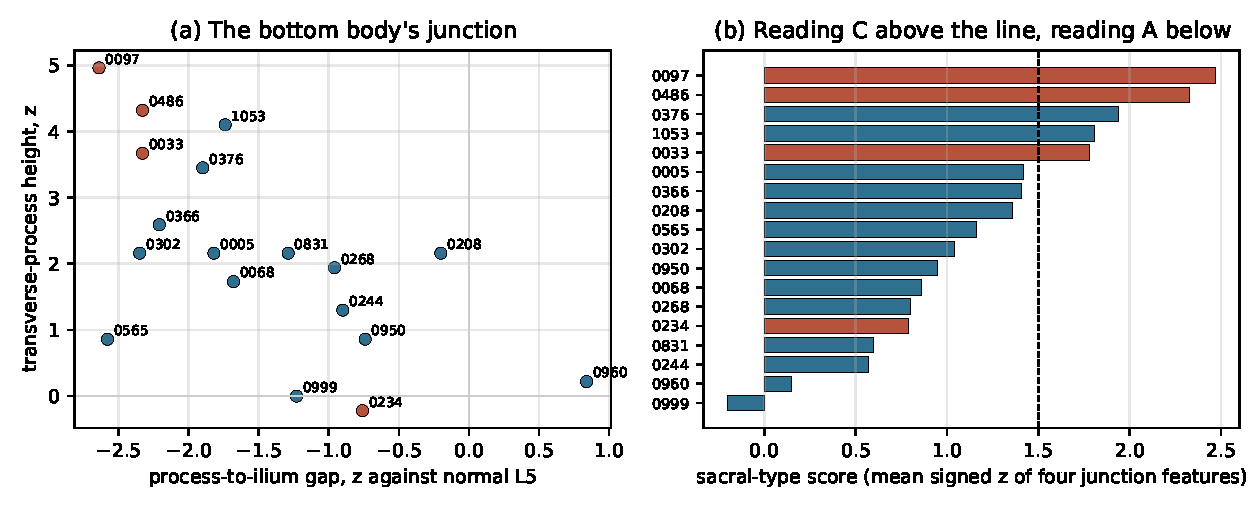
\includegraphics[width=\linewidth]{figs/six_lumbar_readings.pdf}
\caption{The bottom body of each six-lumbar record.
(a)~Transverse-process height against process-to-ilium
gap, as $z$ against normal L5. (b)~The sacral-type score;
records above the line read as a lumbarized S1. Colour is
the final reading after the column-wide shift test.}
\label{fig:sixlumbar}
\end{figure}

\textbf{The bottom body.} Four junction features signed
toward the sacral type (a taller transverse process, a
smaller process-to-ilium gap, a thinner disc beneath, a
shorter sacrum) give a sacral-type score. Six records
exceed 1.5 or carry a sacrum two standard deviations
short; their processes sit 2--5\,SD taller than a normal
L5's and 2\,SD closer to the ilium. Their Castellvi grades
are IIa, IIb, IIb, IIb, IIIb and IV. Because a bilaterally
fused process is carried inside the sacrum label, the
process features go blind exactly at grade III, which is
why sacral height is in the score.

\textbf{The top body.} Rib length cannot see an aplastic
twelfth rib: the labels define the lowest rib-bearing
vertebra as T12, so a spine whose true T12 has no ribs
gets its T11 ribs called ``rib 12'' and every ratio looks
normal. The test is therefore put to the bodies. Each
level of each column is scored under per-level shape
models fitted on the normal records, once as labelled and
once with every name moved up one; on normal controls the
as-labelled reading wins in 37 of 40 with a floor near
$-4$ log-likelihood units. Four six-lumbar records fit
better shifted up, their labelled L1 being a better T12
than L1.

\textbf{Readings.} 11 records read as a true L6, 4 as a
lumbarized S1, 1 (an instrumented record) as an
aplastic-rib T12, and 2 carry evidence at both ends,
which is a real anatomy (a presacral count of 25 with a
rib-less T12) that the field of view cannot exclude. That
last pair is the case for a posterior rather than a
verdict, and it is what the decoder reports.

\textbf{Do the two borders shift together?} Stump twelfth
ribs (length below a third of the eleventh) occur in 98 of
788 records and lumbar ribs in 16 of 802. Among the 14
sacralizations, 4 carry a stump rib against 94 of 758
elsewhere (odds ratio 2.8, $p{=}0.09$); no lumbar rib
occurs among the 14 lumbarizations. The direction agrees
with Nagata et~al.\ (2025); the power does not, at 33
graded records, and the whole-cohort Castellvi read that
would settle it is in progress.

\subsection{The One-Shot Folds}
\label{sec:oneshot-results}

\textbf{[PENDING: five folds launched 7 September 2026;
expected complete about 12 September. To fill from
\texttt{tools/eval\_oneshot.py} and
\texttt{tools/decode\_sequence.py}: (i) per-class Dice on
typical and on transitional records separately; (ii)
rib-free count accuracy by transitional status and the
calibration of the decoder's posterior; (iii) where
ground-truth twelfth-rib, thirteenth-rib and lumbar-rib
voxels went, with lumbar-rib and T13 recall; (iv) the
decoder's readings on the 18 six-lumbar records against
\S\ref{sec:sixlumbar}.]}

% ============================================================================
\section{Discussion and Future Work}
\label{sec:discussion}

\paragraph{Generalization and hardware.}
Any spine segmentation model lacking an L6 class will
exhibit the level-shift on lumbarization; the LSTV gap is
the symptom, not a model-specific bug. Our 100\,GB patch
budget requires H200-class hardware; smaller budgets yield
weaker gap closure and therefore residual wrong-level risk
downstream.

\paragraph{What the readings say about development.}
The 18 six-lumbar spines put the extra segment at the
lumbosacral end (a true L6 or a lumbarized S1) far more
often than at the thoracolumbar end, and the two records
with evidence at both ends are the anatomy a single
homeotic shift of the whole column
predicts~\citep{DuPlessis2018Homeotic,Poolman2023TransitionalVertebrae}.
The stump-rib and sacralization co-occurrence points the
same way at low power. \VerSe{}~\citep{Sekuboyina2021VerSe:Images},
460 volumes with an L6 label and no pelvis, is the
cohort on which the one-shot network and the decoder can
test the shift hypothesis at scale, once our sacral
segmentation (DSC $0.969 \pm 0.002$, 5-fold) supplies the
missing pelvis as a pseudolabel.

\paragraph{What it means at the table.}
Whether the bottom body is an L6 or a lumbarized S1
decides which junction is mobile, how large the pedicle
is and where its trajectory runs, which nerve root exits
beneath it, and which endplate the pelvic parameters were
measured from. A segmenter that reports the type of the
border body with a calibrated posterior gives the surgeon
the one number the count cannot.

\paragraph{Limitations.}
\label{sec:limits-test-set}
COLONOG is a US screening cohort (ages 45--75);
generalization to emergency/pediatric populations is not
evaluated. LSTV labels are inherited from CTPelvic1K and
CTSpine1K heuristics; Castellvi annotation covers all 33
LSTV cases but does not screen the \texttt{normal} cohort
for Type~I, and the source-dataset construction biases
against morphologically-mild Type~I presentations
(\S\ref{sec:castellvi}). The held-out test split contains
7 of the 33 LSTV cases (3 lumb, 1 sacr\_count, 2
sacralization-morph, 1 ambiguous, 0 semi-sacralization);
fold-level evaluation pools across the same 174-case test
set, yielding 15 case-fold pairs for lumbarization and 5
for sacr\_count in voxel-confusion analysis but only the
test-split $n$ for case-level Dice (voxels within a case
are highly correlated, so voxel counts in
\S\ref{sec:residual} represent dependent observations
rather than independent samples). We do not run a
same-compute unmerged 9-class baseline as a controlled
ablation of the merge contribution; the merge's role is
inferred from comparison to \sota{} (which has no L6
class) rather than a same-data ablation. \sota{} is
evaluated zero-shot, the correct comparison for using
\sota{} as a production system but undersells what it
could achieve if retrained with an L6 class.

\paragraph{Implications.}
A production CT segmentation system that emits a
confident, locally well-formed, caudally-shifted prediction
on a 5--35\%-prevalence congenital variant produces no
error signal at inference time and, when consumed
downstream, reproduces the canonical mechanism of
wrong-level spine surgery. Any future spine segmentation
model claiming readiness for surgical-planning integration
should report per-subgroup DSC and per-class confusion at
the L5/S1 junction on a stratified LSTV cohort.

% ============================================================================
\section*{Data and Code Availability}

\dataset{} is hosted on HuggingFace Datasets at
\url{https://huggingface.co/datasets/anonymous-neurips-ED/CTSpinoPelvic1K}
with both core and Responsible AI fields of the
Croissant specification~\citep{Akhtar2024Croissant:Datasets};
a 50-record sample covering all six LSTV subtypes is
available at
\url{https://huggingface.co/datasets/anonymous-neurips-ED/CTSpinoPelvic1K-Sample}.
The evaluation protocol, data-construction pipeline, and
trainer source are released under permissive license at
\url{https://github.com/anonymous-neurips-ED/spinopelvic-seg},
accessible without credentialed access. Trained 5-fold
checkpoints will be made available. All repositories are
anonymized for double-blind review.

\bibliographystyle{plainnat}
\bibliography{bib/references}

\newpage
\section*{NeurIPS Paper Checklist}

%%% BEGIN INSTRUCTIONS %%%
The checklist is designed to encourage best practices for responsible machine learning research, addressing issues of reproducibility, transparency, research ethics, and societal impact. Do not remove the checklist: {\bf The papers not including the checklist will be desk rejected.} The checklist should follow the references and follow the (optional) supplemental material.  The checklist does NOT count towards the page
limit. 

Please read the checklist guidelines carefully for information on how to answer these questions. For each question in the checklist:
\begin{itemize}
    \item You should answer \answerYes{}, \answerNo{}, or \answerNA{}.
    \item \answerNA{} means either that the question is Not Applicable for that particular paper or the relevant information is Not Available.
    \item Please provide a short (1--2 sentence) justification right after your answer (even for \answerNA). 
   % \item {\bf The papers not including the checklist will be desk rejected.}
\end{itemize}

{\bf The checklist answers are an integral part of your paper submission.} They are visible to the reviewers, area chairs, senior area chairs, and ethics reviewers. You will also be asked to include it (after eventual revisions) with the final version of your paper, and its final version will be published with the paper.

The reviewers of your paper will be asked to use the checklist as one of the factors in their evaluation. While \answerYes{} is generally preferable to \answerNo{}, it is perfectly acceptable to answer \answerNo{} provided a proper justification is given (e.g., error bars are not reported because it would be too computationally expensive'' or ``we were unable to find the license for the dataset we used''). In general, answering \answerNo{} or \answerNA{} is not grounds for rejection. While the questions are phrased in a binary way, we acknowledge that the true answer is often more nuanced, so please just use your best judgment and write a justification to elaborate. All supporting evidence can appear either in the main paper or the supplemental material, provided in appendix. If you answer \answerYes{} to a question, in the justification please point to the section(s) where related material for the question can be found.

IMPORTANT, please:
\begin{itemize}
    \item {\bf Delete this instruction block, but keep the section heading ``NeurIPS Paper Checklist"},
    \item  {\bf Keep the checklist subsection headings, questions/answers and guidelines below.}
    \item {\bf Do not modify the questions and only use the provided macros for your answers}.
\end{itemize} 
 

%%% END INSTRUCTIONS %%%


\begin{enumerate}

\item {\bf Claims}
    \item[] Question: Do the main claims made in the abstract and introduction accurately reflect the paper's contributions and scope?
    \item[] Answer: \answerTODO{} % Replace by \answerYes{}, \answerNo{}, or \answerNA{}.
    \item[] Justification: \justificationTODO{}
    \item[] Guidelines:
    \begin{itemize}
        \item The answer \answerNA{} means that the abstract and introduction do not include the claims made in the paper.
        \item The abstract and/or introduction should clearly state the claims made, including the contributions made in the paper and important assumptions and limitations. A \answerNo{} or \answerNA{} answer to this question will not be perceived well by the reviewers. 
        \item The claims made should match theoretical and experimental results, and reflect how much the results can be expected to generalize to other settings. 
        \item It is fine to include aspirational goals as motivation as long as it is clear that these goals are not attained by the paper. 
    \end{itemize}

\item {\bf Limitations}
    \item[] Question: Does the paper discuss the limitations of the work performed by the authors?
    \item[] Answer: \answerTODO{} % Replace by \answerYes{}, \answerNo{}, or \answerNA{}.
    \item[] Justification: \justificationTODO{}
    \item[] Guidelines:
    \begin{itemize}
        \item The answer \answerNA{} means that the paper has no limitation while the answer \answerNo{} means that the paper has limitations, but those are not discussed in the paper. 
        \item The authors are encouraged to create a separate ``Limitations'' section in their paper.
        \item The paper should point out any strong assumptions and how robust the results are to violations of these assumptions (e.g., independence assumptions, noiseless settings, model well-specification, asymptotic approximations only holding locally). The authors should reflect on how these assumptions might be violated in practice and what the implications would be.
        \item The authors should reflect on the scope of the claims made, e.g., if the approach was only tested on a few datasets or with a few runs. In general, empirical results often depend on implicit assumptions, which should be articulated.
        \item The authors should reflect on the factors that influence the performance of the approach. For example, a facial recognition algorithm may perform poorly when image resolution is low or images are taken in low lighting. Or a speech-to-text system might not be used reliably to provide closed captions for online lectures because it fails to handle technical jargon.
        \item The authors should discuss the computational efficiency of the proposed algorithms and how they scale with dataset size.
        \item If applicable, the authors should discuss possible limitations of their approach to address problems of privacy and fairness.
        \item While the authors might fear that complete honesty about limitations might be used by reviewers as grounds for rejection, a worse outcome might be that reviewers discover limitations that aren't acknowledged in the paper. The authors should use their best judgment and recognize that individual actions in favor of transparency play an important role in developing norms that preserve the integrity of the community. Reviewers will be specifically instructed to not penalize honesty concerning limitations.
    \end{itemize}

\item {\bf Theory assumptions and proofs}
    \item[] Question: For each theoretical result, does the paper provide the full set of assumptions and a complete (and correct) proof?
    \item[] Answer: \answerTODO{} % Replace by \answerYes{}, \answerNo{}, or \answerNA{}.
    \item[] Justification: \justificationTODO{}
    \item[] Guidelines:
    \begin{itemize}
        \item The answer \answerNA{} means that the paper does not include theoretical results. 
        \item All the theorems, formulas, and proofs in the paper should be numbered and cross-referenced.
        \item All assumptions should be clearly stated or referenced in the statement of any theorems.
        \item The proofs can either appear in the main paper or the supplemental material, but if they appear in the supplemental material, the authors are encouraged to provide a short proof sketch to provide intuition. 
        \item Inversely, any informal proof provided in the core of the paper should be complemented by formal proofs provided in appendix or supplemental material.
        \item Theorems and Lemmas that the proof relies upon should be properly referenced. 
    \end{itemize}

    \item {\bf Experimental result reproducibility}
    \item[] Question: Does the paper fully disclose all the information needed to reproduce the main experimental results of the paper to the extent that it affects the main claims and/or conclusions of the paper (regardless of whether the code and data are provided or not)?
    \item[] Answer: \answerTODO{} % Replace by \answerYes{}, \answerNo{}, or \answerNA{}.
    \item[] Justification: \justificationTODO{}
    \item[] Guidelines:
    \begin{itemize}
        \item The answer \answerNA{} means that the paper does not include experiments.
        \item If the paper includes experiments, a \answerNo{} answer to this question will not be perceived well by the reviewers: Making the paper reproducible is important, regardless of whether the code and data are provided or not.
        \item If the contribution is a dataset and\slash or model, the authors should describe the steps taken to make their results reproducible or verifiable. 
        \item Depending on the contribution, reproducibility can be accomplished in various ways. For example, if the contribution is a novel architecture, describing the architecture fully might suffice, or if the contribution is a specific model and empirical evaluation, it may be necessary to either make it possible for others to replicate the model with the same dataset, or provide access to the model. In general. releasing code and data is often one good way to accomplish this, but reproducibility can also be provided via detailed instructions for how to replicate the results, access to a hosted model (e.g., in the case of a large language model), releasing of a model checkpoint, or other means that are appropriate to the research performed.
        \item While NeurIPS does not require releasing code, the conference does require all submissions to provide some reasonable avenue for reproducibility, which may depend on the nature of the contribution. For example
        \begin{enumerate}
            \item If the contribution is primarily a new algorithm, the paper should make it clear how to reproduce that algorithm.
            \item If the contribution is primarily a new model architecture, the paper should describe the architecture clearly and fully.
            \item If the contribution is a new model (e.g., a large language model), then there should either be a way to access this model for reproducing the results or a way to reproduce the model (e.g., with an open-source dataset or instructions for how to construct the dataset).
            \item We recognize that reproducibility may be tricky in some cases, in which case authors are welcome to describe the particular way they provide for reproducibility. In the case of closed-source models, it may be that access to the model is limited in some way (e.g., to registered users), but it should be possible for other researchers to have some path to reproducing or verifying the results.
        \end{enumerate}
    \end{itemize}


\item {\bf Open access to data and code}
    \item[] Question: Does the paper provide open access to the data and code, with sufficient instructions to faithfully reproduce the main experimental results, as described in supplemental material?
    \item[] Answer: \answerTODO{} % Replace by \answerYes{}, \answerNo{}, or \answerNA{}.
    \item[] Justification: \justificationTODO{}
    \item[] Guidelines:
    \begin{itemize}
        \item The answer \answerNA{} means that paper does not include experiments requiring code.
        \item Please see the NeurIPS code and data submission guidelines (\url{https://neurips.cc/public/guides/CodeSubmissionPolicy}) for more details.
        \item While we encourage the release of code and data, we understand that this might not be possible, so \answerNo{} is an acceptable answer. Papers cannot be rejected simply for not including code, unless this is central to the contribution (e.g., for a new open-source benchmark).
        \item The instructions should contain the exact command and environment needed to run to reproduce the results. See the NeurIPS code and data submission guidelines (\url{https://neurips.cc/public/guides/CodeSubmissionPolicy}) for more details.
        \item The authors should provide instructions on data access and preparation, including how to access the raw data, preprocessed data, intermediate data, and generated data, etc.
        \item The authors should provide scripts to reproduce all experimental results for the new proposed method and baselines. If only a subset of experiments are reproducible, they should state which ones are omitted from the script and why.
        \item At submission time, to preserve anonymity, the authors should release anonymized versions (if applicable).
        \item Providing as much information as possible in supplemental material (appended to the paper) is recommended, but including URLs to data and code is permitted.
    \end{itemize}


\item {\bf Experimental setting/details}
    \item[] Question: Does the paper specify all the training and test details (e.g., data splits, hyperparameters, how they were chosen, type of optimizer) necessary to understand the results?
    \item[] Answer: \answerTODO{} % Replace by \answerYes{}, \answerNo{}, or \answerNA{}.
    \item[] Justification: \justificationTODO{}
    \item[] Guidelines:
    \begin{itemize}
        \item The answer \answerNA{} means that the paper does not include experiments.
        \item The experimental setting should be presented in the core of the paper to a level of detail that is necessary to appreciate the results and make sense of them.
        \item The full details can be provided either with the code, in appendix, or as supplemental material.
    \end{itemize}

\item {\bf Experiment statistical significance}
    \item[] Question: Does the paper report error bars suitably and correctly defined or other appropriate information about the statistical significance of the experiments?
    \item[] Answer: \answerTODO{} % Replace by \answerYes{}, \answerNo{}, or \answerNA{}.
    \item[] Justification: \justificationTODO{}
    \item[] Guidelines:
    \begin{itemize}
        \item The answer \answerNA{} means that the paper does not include experiments.
        \item The authors should answer \answerYes{} if the results are accompanied by error bars, confidence intervals, or statistical significance tests, at least for the experiments that support the main claims of the paper.
        \item The factors of variability that the error bars are capturing should be clearly stated (for example, train/test split, initialization, random drawing of some parameter, or overall run with given experimental conditions).
        \item The method for calculating the error bars should be explained (closed form formula, call to a library function, bootstrap, etc.)
        \item The assumptions made should be given (e.g., Normally distributed errors).
        \item It should be clear whether the error bar is the standard deviation or the standard error of the mean.
        \item It is OK to report 1-sigma error bars, but one should state it. The authors should preferably report a 2-sigma error bar than state that they have a 96\% CI, if the hypothesis of Normality of errors is not verified.
        \item For asymmetric distributions, the authors should be careful not to show in tables or figures symmetric error bars that would yield results that are out of range (e.g., negative error rates).
        \item If error bars are reported in tables or plots, the authors should explain in the text how they were calculated and reference the corresponding figures or tables in the text.
    \end{itemize}

\item {\bf Experiments compute resources}
    \item[] Question: For each experiment, does the paper provide sufficient information on the computer resources (type of compute workers, memory, time of execution) needed to reproduce the experiments?
    \item[] Answer: \answerTODO{} % Replace by \answerYes{}, \answerNo{}, or \answerNA{}.
    \item[] Justification: \justificationTODO{}
    \item[] Guidelines:
    \begin{itemize}
        \item The answer \answerNA{} means that the paper does not include experiments.
        \item The paper should indicate the type of compute workers CPU or GPU, internal cluster, or cloud provider, including relevant memory and storage.
        \item The paper should provide the amount of compute required for each of the individual experimental runs as well as estimate the total compute. 
        \item The paper should disclose whether the full research project required more compute than the experiments reported in the paper (e.g., preliminary or failed experiments that didn't make it into the paper). 
    \end{itemize}
    
\item {\bf Code of ethics}
    \item[] Question: Does the research conducted in the paper conform, in every respect, with the NeurIPS Code of Ethics \url{https://neurips.cc/public/EthicsGuidelines}?
    \item[] Answer: \answerTODO{} % Replace by \answerYes{}, \answerNo{}, or \answerNA{}.
    \item[] Justification: \justificationTODO{}
    \item[] Guidelines:
    \begin{itemize}
        \item The answer \answerNA{} means that the authors have not reviewed the NeurIPS Code of Ethics.
        \item If the authors answer \answerNo, they should explain the special circumstances that require a deviation from the Code of Ethics.
        \item The authors should make sure to preserve anonymity (e.g., if there is a special consideration due to laws or regulations in their jurisdiction).
    \end{itemize}


\item {\bf Broader impacts}
    \item[] Question: Does the paper discuss both potential positive societal impacts and negative societal impacts of the work performed?
    \item[] Answer: \answerTODO{} % Replace by \answerYes{}, \answerNo{}, or \answerNA{}.
    \item[] Justification: \justificationTODO{}
    \item[] Guidelines:
    \begin{itemize}
        \item The answer \answerNA{} means that there is no societal impact of the work performed.
        \item If the authors answer \answerNA{} or \answerNo, they should explain why their work has no societal impact or why the paper does not address societal impact.
        \item Examples of negative societal impacts include potential malicious or unintended uses (e.g., disinformation, generating fake profiles, surveillance), fairness considerations (e.g., deployment of technologies that could make decisions that unfairly impact specific groups), privacy considerations, and security considerations.
        \item The conference expects that many papers will be foundational research and not tied to particular applications, let alone deployments. However, if there is a direct path to any negative applications, the authors should point it out. For example, it is legitimate to point out that an improvement in the quality of generative models could be used to generate Deepfakes for disinformation. On the other hand, it is not needed to point out that a generic algorithm for optimizing neural networks could enable people to train models that generate Deepfakes faster.
        \item The authors should consider possible harms that could arise when the technology is being used as intended and functioning correctly, harms that could arise when the technology is being used as intended but gives incorrect results, and harms following from (intentional or unintentional) misuse of the technology.
        \item If there are negative societal impacts, the authors could also discuss possible mitigation strategies (e.g., gated release of models, providing defenses in addition to attacks, mechanisms for monitoring misuse, mechanisms to monitor how a system learns from feedback over time, improving the efficiency and accessibility of ML).
    \end{itemize}
    
\item {\bf Safeguards}
    \item[] Question: Does the paper describe safeguards that have been put in place for responsible release of data or models that have a high risk for misuse (e.g., pre-trained language models, image generators, or scraped datasets)?
    \item[] Answer: \answerTODO{} % Replace by \answerYes{}, \answerNo{}, or \answerNA{}.
    \item[] Justification: \justificationTODO{}
    \item[] Guidelines:
    \begin{itemize}
        \item The answer \answerNA{} means that the paper poses no such risks.
        \item Released models that have a high risk for misuse or dual-use should be released with necessary safeguards to allow for controlled use of the model, for example by requiring that users adhere to usage guidelines or restrictions to access the model or implementing safety filters. 
        \item Datasets that have been scraped from the Internet could pose safety risks. The authors should describe how they avoided releasing unsafe images.
        \item We recognize that providing effective safeguards is challenging, and many papers do not require this, but we encourage authors to take this into account and make a best faith effort.
    \end{itemize}

\item {\bf Licenses for existing assets}
    \item[] Question: Are the creators or original owners of assets (e.g., code, data, models), used in the paper, properly credited and are the license and terms of use explicitly mentioned and properly respected?
    \item[] Answer: \answerTODO{} % Replace by \answerYes{}, \answerNo{}, or \answerNA{}.
    \item[] Justification: \justificationTODO{}
    \item[] Guidelines:
    \begin{itemize}
        \item The answer \answerNA{} means that the paper does not use existing assets.
        \item The authors should cite the original paper that produced the code package or dataset.
        \item The authors should state which version of the asset is used and, if possible, include a URL.
        \item The name of the license (e.g., CC-BY 4.0) should be included for each asset.
        \item For scraped data from a particular source (e.g., website), the copyright and terms of service of that source should be provided.
        \item If assets are released, the license, copyright information, and terms of use in the package should be provided. For popular datasets, \url{paperswithcode.com/datasets} has curated licenses for some datasets. Their licensing guide can help determine the license of a dataset.
        \item For existing datasets that are re-packaged, both the original license and the license of the derived asset (if it has changed) should be provided.
        \item If this information is not available online, the authors are encouraged to reach out to the asset's creators.
    \end{itemize}

\item {\bf New assets}
    \item[] Question: Are new assets introduced in the paper well documented and is the documentation provided alongside the assets?
    \item[] Answer: \answerTODO{} % Replace by \answerYes{}, \answerNo{}, or \answerNA{}.
    \item[] Justification: \justificationTODO{}
    \item[] Guidelines:
    \begin{itemize}
        \item The answer \answerNA{} means that the paper does not release new assets.
        \item Researchers should communicate the details of the dataset\slash code\slash model as part of their submissions via structured templates. This includes details about training, license, limitations, etc. 
        \item The paper should discuss whether and how consent was obtained from people whose asset is used.
        \item At submission time, remember to anonymize your assets (if applicable). You can either create an anonymized URL or include an anonymized zip file.
    \end{itemize}

\item {\bf Crowdsourcing and research with human subjects}
    \item[] Question: For crowdsourcing experiments and research with human subjects, does the paper include the full text of instructions given to participants and screenshots, if applicable, as well as details about compensation (if any)? 
    \item[] Answer: \answerTODO{} % Replace by \answerYes{}, \answerNo{}, or \answerNA{}.
    \item[] Justification: \justificationTODO{}
    \item[] Guidelines:
    \begin{itemize}
        \item The answer \answerNA{} means that the paper does not involve crowdsourcing nor research with human subjects.
        \item Including this information in the supplemental material is fine, but if the main contribution of the paper involves human subjects, then as much detail as possible should be included in the main paper. 
        \item According to the NeurIPS Code of Ethics, workers involved in data collection, curation, or other labor should be paid at least the minimum wage in the country of the data collector. 
    \end{itemize}

\item {\bf Institutional review board (IRB) approvals or equivalent for research with human subjects}
    \item[] Question: Does the paper describe potential risks incurred by study participants, whether such risks were disclosed to the subjects, and whether Institutional Review Board (IRB) approvals (or an equivalent approval/review based on the requirements of your country or institution) were obtained?
    \item[] Answer: \answerTODO{} % Replace by \answerYes{}, \answerNo{}, or \answerNA{}.
    \item[] Justification: \justificationTODO{}
    \item[] Guidelines:
    \begin{itemize}
        \item The answer \answerNA{} means that the paper does not involve crowdsourcing nor research with human subjects.
        \item Depending on the country in which research is conducted, IRB approval (or equivalent) may be required for any human subjects research. If you obtained IRB approval, you should clearly state this in the paper. 
        \item We recognize that the procedures for this may vary significantly between institutions and locations, and we expect authors to adhere to the NeurIPS Code of Ethics and the guidelines for their institution. 
        \item For initial submissions, do not include any information that would break anonymity (if applicable), such as the institution conducting the review.
    \end{itemize}

\item {\bf Declaration of LLM usage}
    \item[] Question: Does the paper describe the usage of LLMs if it is an important, original, or non-standard component of the core methods in this research? Note that if the LLM is used only for writing, editing, or formatting purposes and does \emph{not} impact the core methodology, scientific rigor, or originality of the research, declaration is not required.
    %this research? 
    \item[] Answer: \answerTODO{} % Replace by \answerYes{}, \answerNo{}, or \answerNA{}.
    \item[] Justification: \justificationTODO{}
    \item[] Guidelines:
    \begin{itemize}
        \item The answer \answerNA{} means that the core method development in this research does not involve LLMs as any important, original, or non-standard components.
        \item Please refer to our LLM policy in the NeurIPS handbook for what should or should not be described.
    \end{itemize}

\end{enumerate}

\end{document}
